% Modified from AAAS Science LATEX template
% Use only LaTeX2e, calling the article.cls class and 12-point type.

\documentclass[11pt, a4paper, oneside]{article}
\usepackage{helvet}
\renewcommand{\familydefault}{\sfdefault}

\usepackage{graphicx}

\usepackage{caption}
\captionsetup{font=small}
\usepackage{url}

\usepackage{scicite}

% Page setup

\topmargin 0.0cm
\oddsidemargin 0.2cm
\textwidth 16cm
\textheight 21cm
\footskip 1.0cm

\usepackage[legalpaper, portrait, margin=0.5in]{geometry}

\newcommand{\beginsupplement}{%
  \setcounter{table}{0}
  \renewcommand{\thetable}{S\arabic{table}}%
  \setcounter{figure}{0}
  \renewcommand{\thefigure}{S\arabic{figure}}%
}

% Abstract environment
\newenvironment{sciabstract}{%
\begin{quote} \bf}
{\end{quote}}

% Paper title
\title{
XPRESSyourself: Automating and Democratizing High-Throughput Sequencing
}

% Author info
\author{
% Tentative author list/order:
%Jordan A. Berg,$^{1}$ Jeffrey T. Morgan,$^{1}$ Jonathan R. Belyeu,$^{2}$ Alex J. Bott,$^{1}$ Yeyun Ouyang,$^{1}$\\
%Aaron R. Quinlan,$^{2,4,5}$ Jason Gertz,$^{3}$ Michael T. Howard,$^{2}$ Jared P. Rutter$^{1,6\ast}$\\
%\\
%\normalsize{$^{1}$Department of Biochemistry, University of Utah, Salt Lake City, UT, USA, 84112}\\
%\normalsize{$^{2}$Department of Human Genetics, University of Utah, Salt Lake City, UT, USA, 84112}\\
%\normalsize{$^{3}$Department of Oncological Sciences, University of Utah, Salt Lake City, UT, USA, 84112}\\
%\normalsize{$^{4}$USTAR Center for Genetic Discovery, University of Utah, Salt Lake City, UT, USA, 84112}\\
%\normalsize{$^{5}$Department of Biomedical Informatics, University of Utah, Salt Lake City, UT, USA, 84112}\\
%\normalsize{$^{6}$Howard Hughes Medical Institute, University of Utah, Salt Lake City, UT, USA, 84112}\\
%\\
%\normalsize{$^\ast$To whom correspondence should be addressed; E-mail: rutter@biochem.utah.edu.}
}

% Include the date command, but leave its argument blank.
\date{}

%%%%%%%%%%%%%%%%% END OF PREAMBLE %%%%%%%%%%%%%%%%


% Initialize use of code blocks with syntax highlighting

\usepackage{listings}
\usepackage{color}

\definecolor{dkgreen}{rgb}{0,0.6,0}
\definecolor{gray}{rgb}{0.5,0.5,0.5}
\definecolor{mauve}{rgb}{0.58,0,0.82}

\lstset{frame=tb,
  language=Java,
  aboveskip=3mm,
  belowskip=3mm,
  showstringspaces=false,
  columns=flexible,
  basicstyle={\small\ttfamily},
  numbers=none,
  numberstyle=\tiny\color{gray},
  keywordstyle=\color{blue},
  commentstyle=\color{dkgreen},
  stringstyle=\color{mauve},
  breaklines=true,
  breakatwhitespace=true,
  tabsize=3
}


\begin{document}

% Double-space the manuscript.
\baselineskip24pt

% Make the title.
\maketitle



% Place your abstract within the special {sciabstract} environment.
\begin{sciabstract}
Sequencing experiments are routine and often necessary in biological and clinical research. However, for the average user, a computational overhead often exists. XPRESSyourself is a ribosome profiling and general RNA-seq pipeline that aims to eliminate these barriers, standardize \textit{in silico} protocols, and decrease time-to-discovery from data. With these tools, a user can go from raw data to publication quality figures in a matter of hours. Additionally, XPRESSyourself introduces tools missing from the ribosome profiling and RNA-seq computational toolkit. Using XPRESSyourself, we discovered new putative hits from publicly available ribosome profiling data, highlighting its utility to reveal biological insight.
\end{sciabstract}

\section*{Keywords}
Pipeline, Ribosome Profiling, RNA-seq, Automation, Standardization

\section{Background}
High-throughput profiling of gene expression data has revolutionized biomedical, industrial, and basic science research. Within the last two decades, RNA-seq has found itself the forerunner technology for high quality gene expression profiling, as it can measure relative transcript abundance, differential splice variants, sequence polymorphisms, and more \cite{byron_nrg}. This technology has been co-opted to create a variety of technologies such as single-cell RNA-seq, ChIP-seq, and ribosome profiling \cite{ingolia_science}. \par

While vast strides have been made to these technologies, various bottlenecks still exist. For example, while more and more researchers are becoming accustomed to to the field of bioinformatics and computational biology, learning the intricracies of the different tools used in processing RNA-seq data can be inhibitory if users are not aware of the proper tools to use or use outdated software \cite{costello_npjsba, funari_science}. Even for the experienced user, developing robust, automated pipelines that meticulously process and assess quality of these datasets can be laborious, notwithstanding the induced variability that comes with each lab or bioinformatics core designing and using their own pipelines. \par

While RNA-seq is a more matured technology, there are still an abundance of biases and idiosyncrasies associated with each method or tool of which the beginner user may not be aware. Additionally, few if any pre-existing pipeline or toolkit offer a thorough set of integrated tools for handling common quality control issues or reference creation. For example, a common bias in ribosome profiling libraries is a 5' transcript pile-up \cite{gerashchenko_nar, artieri_gr, hussman_plosg}. It is recommended that this region of each transcript not be quantified when processing ribosome profiling libraries; however, currently no tools exist to facilitate this essential step \cite{ingolia_meth, weinberg_reports}. \par

Several computational pipelines for sequencing have emerged intending to tackle various aspects of these bottlenecks, but many suffer from usability issues, are not easily modifiable, or sacrifice quality for speed. For example, a simple internet search for RNA-seq pipelines will reveal several classes of pipeline. The first class is a tutorial titled a pipeline. Many instances of these can be found (https://www.encodeproject.org/rna-seq/, https://docs.gdc.cancer.gov/Data/Bioinformatics\_Pipelines/Expression\_mRNA\_Pipeline/); however, they are not automated and are often outdated. The second class is an automated pipeline, but requires extensive manual configuration (https://github.com/PavlidisLab/rnaseq-pipeline, https://github.com/nf-core/rnaseq, https://github.com/UMCUGenetics/RNASeq, https://github.com/cellgeni/rnaseq). The second class is an automated pipeline, but requires programmatic configuration to modify common parameters (https://github.com/dnanexus/tophat\_cufflinks\_rnaseq, https://www.nextflow.io/example4.html). Perhaps, the most user friendly case is Galaxy, but in cases like its ribosome profiling pipeline, methods are severly outdated and a robust quality control step is lacking. In all cases, a thorough, robust, simple pipeline geared to the general user without sacrificing for speed or quality is lacking. \par

In response to the issues surrounding the automation and democratization of sequencing technology, we designed the XPRESSyourself bioinformatics suite for processing and analyzing high-throughput expression data. Architectually, this suite is designed to work fast, while not sacrificing quality for speed. Each step of the pipelines utilize the state of the art software package for that task, having been previously vetted by peer-reviewed benchmarking studies. Additionally, the scaffold that creates this pipeline structure is designed in a way that update and testing of a new module when better software comes along should only take a couple of hours for a trained bioinformatician, thus making the best options available to the community at large, especially for those that may not be aware of such updates. \par

With the XPRESSyourself package XPRESSpipe, the user is provided with a complete suite of software to handle pre-processing, aligning, and quantifying reads, performing quality control via various meta-analyses of pre- and post-processed reads. We also provide access to key quality control measures useful for assessing ribosome profiling and other RNA-seq experiments. These include read length distributions to ensure correct sequencing library read sizes and a periodicity sub-module that tracks the P-site of ribosome footprints to assess effective capture of the ribosome's characteristic 1 codon step. These measurements are particular helpful for ribosome profiling experiments due the unique characteristics of the ribosome footprint-sized libraries (usually around 21-30 nt). XPRESSpipe also includes a metagene analysis sub-module that shows the distribution of all aligned reads across a representative transcript a library and a library complexity visualization sub-module to ensure minimalization of PCR duplicates. Additionally, housed within the XPRESSyourself XPRESSplot package, tools are provided to perform the bulk of sequence analysis and generation of figures for publication, where many plot generation protocols that might take several hundred lines of code are whittled down to one line. XPRESSyourself suite tools are perpetually open source under a GPL-3.0 license at https://github.com/XPRESSyourself.


\section{Results}

\subsection{XPRESSpipe}
XPRESSpipe contains automated pipelines for ribosome profiling, single-end, and paired-end RNA-seq. Each pipeline offers a selection of tunable parameters most pertinent to the user. The pipeline requirements are also largely based upon The Cancer Genome Atlas (TCGA) (https://www.cancer.gov/tcga) alignment standards and ensure standardization of alignment. In the future it is feasible that additional tunable parameters will be added. For the purposes of this manuscript, we will focus on ribosome profiling examples, while the majority of statements are also applicable to single- and paired-end RNA-seq. More details can be found in the documentation that will be continually updated as features are updated or changed (https://xpresspipe.readthedocs.io/en/latest/). Table \ref{Tab:xpresspipe} outlines these parameters.

\captionof{table}{Summary of XPRESSpipe pipeline arguments.\label{Tab:xpresspipe}}
\begin{tabular}{p{5cm}p{13cm}}
 \textbf{Arguments} & \textbf{Description} \\
 \hline
 \textbf{Required} & \\
 \hline
 \texttt{-i, --input} & Path to input directory \\
 \hline
 \texttt{-o, --output} & Path to output directory \\
 \hline
 \texttt{-r, --reference} & Path to parent organism reference directory \\
 \hline
 \texttt{-g, --gtf} & Path and file name to GTF used for alignment quantification \\
 \hline
 \texttt{-e, --experiment} & Experiment name \\
 \hline
 \textbf{Optional} & \\
 \hline
 \texttt{--two\_pass} & Include option to perform a two-step alignment to map for unannotated splice-juntions \\
 \hline
 \texttt{-a, --adaptors} & Specify adaptor as string -- if ``None" is provided, software will attempt to auto-detect adaptors -- if ``POLYX" is provided as a single string in the list, polyX adaptors will be trimmed \\
 \hline
 \texttt{-q, --quality} & PHRED read quality threshold (default: 28) \\
 \hline
 \texttt{--min\_length} & Minimum read length threshold to keep for reads (default: 18) \\
 \hline
 \texttt{--count\_duplicates} & Include option to quantify alignment files without de-duplication \\
 \hline
 \texttt{--output\_bed} & Include option to output BED files for each aligned file \\
 \hline
 \texttt{--output\_bigwig} & Include flag to output bigwig files for each aligned file \\
 \hline
 \texttt{-c, --quantification\_method} & Specify quantification method (default: HTSeq-count\cite{htseq}) \\
 \hline
 \texttt{--method} & Normalization method to perform (options: ``RPM", ``TPM", ``RPKM", ``FPKM") \\
 \hline
 \texttt{--batch} & Include path and filename of dataframe with batch normalization parameters \\
 \hline
 \texttt{--sjdbOverhang} & Sequencing platform read-length for constructing splice-aware reference previously (see STAR documentation for more information) \\
 \hline
 \texttt{--mismatchRatio} & Alignment ratio of mismatches to mapped length is less than this value (see STAR documentation for more information) \\
 \hline
 \texttt{--seedSearchStartLmax} & Adjusting this parameter by providing a lower number will improve mapping sensitivity (recommended value = 15 for reads ~ 25 nts) (see STAR documentation for more information) \\
 \hline
 \texttt{-m, --max\_processors} & Number of max processors to use for tasks (default: No limit) \\
\end{tabular}
\newline

\subsubsection{Installation}
XPRESSpipe can be compiled from source (https://github.com/XPRESSyourself/XPRESSpipe) or a version-controlled Docker image (https://www.docker.com/) can be loaded using the following commands: \par

% Install XPRESSpipe code block
\begin{lstlisting}[language=bash, caption=Source installation.]
# Download and unzip archived version from https://github.com/XPRESSyourself/XPRESSpipe/releases
$ cd XPRESSpipe
$ python setup.py install
\end{lstlisting}

XPRESSpipe is built upon several pre-established software packages required as dependencies. A full list can be found in the Methods. The source install will automatically check the user's system for Anaconda\cite{anaconda} and install required dependencies. If working on a compute cluster without administrative priveledges, Anaconda should be installed manually first before installing XPRESSpipe and associated dependencies. Anaconda and XPRESSpipe should be directed to the user's \texttt{.local} directory, as follows:

% Install Anaconda code block
\begin{lstlisting}[language=bash, caption=Anaconda installation on compute node.]
# Clean environment of pre-installed dependencies by admins
$ cd $HOME
$ module purge

# Get the latest anaconda3 distribution and make executable
$ curl -O https://repo.anaconda.com/archive/Anaconda3-5.3.0-Linux-x86_64.sh
$ chmod 700 Anaconda3-5.3.0-Linux-x86_64.sh

# Install Anaconda in batch mode (assumes license agreed upon, setup prefix directory, and skip pre- and post- install scripts)
export INSTALL_DIR=$HOME/softwares/anaconda3/5.3.0
./Anaconda3-5.3.0-Linux-x86_64.sh -b -p $INSTALL_DIR -s
\end{lstlisting}


% Install XPRESSpipe code block
\begin{lstlisting}[language=bash, caption=Source installation on compute node.]
# Download and unzip archived version from https://github.com/XPRESSyourself/XPRESSpipe/releases
$ cd XPRESSpipe
$ python setup.py install --prefix ~/.local/bin
\end{lstlisting}

Docker images come with these dependencies pre-installed and can be accessed as follows:

% Install XPRESSpipe code block
\begin{lstlisting}[language=bash, caption=Docker installation]
$ docker image pull jordanberg/xpresspipe:latest
\end{lstlisting}

\subsubsection{Inputs}
While inputs will vary sub-module to sub-module, and further information can be found in the documentation (https://xpresspipe.readthedocs.io/en/latest/) or by entering \texttt{xpresspipe \textless sub-module name\textgreater \ --help}, a few points of guidance are important to consider.

\begin{itemize}
\item Single-end reads should end in \texttt{.fa}, \texttt{.fasta}, or \texttt{.txt}
\item Paired-end reads should end in \texttt{.read1/2.fa} or \texttt{.r1/2.fa}, where \texttt{.fa} could also be \texttt{.fasta} or \texttt{.txt}
\item The base transcriptome reference file should be a valid GTF file and should be named \texttt{transcripts.gtf}
\item If specifying a group of fasta files to use for alignment or reference curation, the directory containing these files cannot contain any other files ending in \texttt{.txt} or \texttt{.fa}
\end{itemize}

\subsubsection{Reference Curation}
One of the first steps of RNA-seq alignment is curating a reference to which the alignment software will map reads. For the purposes of the current version of XPRESSpipe, a STAR \cite{star} reference should be created. An Ensembl-formatted (https://ensembl.org) GTF should also be placed in the reference directory and be named \texttt{transcripts.gtf}. Additional modifications are recommended to this file, which can be performed using this sub-module, discussed in more detail in the next section. Additionally, any chromosome \texttt{.fasta} files should be places in their own directory within the curated reference directory. As this can be a time-consuming process, we will leave the \texttt{--max\_processors} argument as default in order to utilize all cores available to the computing unit. This entire process is handled with the \texttt{curateReference} sub-module for ease of use to the user.
\newline
\begin{lstlisting}[language=bash, caption=curateReference example]
$ xpresspipe curateReference -o /path/to/output/location/ \
                                -f /path/to/fasta/genome/ \
                                -g /path/transcripts.gtf \
                                --protein_coding \
                                --longest_transcript \
                                --truncate \
                                --truncate_5prime 45 \
                                --truncate_3prime 15 \
                                --sjdbOverhang 49 \
                                --max_processors None
\end{lstlisting}


\subsubsection{GTF Modification}
As ribosomal RNAs and other non-coding RNAs are highly abundant in RNA-seq experiments, it is often recommended to disregard these sequences. By providing the \texttt{--protein\_coding} argument, only protein-coding genes are retained in the GTF file, which acts as a masking of any reads aligning to non-coding regions of the genome. \par

In most eukaryotes, mRNAs undergo alternative splicing. However, some quantification will consider the multiply annotated splice variants of a gene as a multi-mapper since they map to a location where several isoforms of the same gene overlap. These reads are either penalized or discarded. By providing the \texttt{--longest\_transcript} argument, the longest coding transcript for each gene is retained in the GTF file. However, if using Cufflinks to quantify reads (discussed further in the next section), this is not recommended as Cufflinks is optimized to quantify isoform abundances \cite{cufflinks}. \par

For the purposes of ribosome profiling, where 5' and 3' transcript biases are frequent \cite{ingolia_meth, weinberg_reports}, the 5' and 3' ends of each transcript record need to be trimmed to avoid quantification to this region. By providing the \texttt{--truncate} argument, the 5' and 3' ends of each transcript will be trimmed by the specified amounts.

\subsubsection{Read Processing}
While all intermediate steps of the pipelines can be run singly, we will describe the outline of the software in the context of the ribosome profiling pipeline. Pipelines and individual sub-modules are capable of being run in a parallel manner for each input file, thus accelerating the overall process. Descriptions of the options can be found in Table \ref{Tab:xpresspipe}.

\begin{enumerate}
  \item \textbf{Trimming}: First, reads need to be cleaned of artifacts from library creation. These include adaptors, unique molecular identifier (UMI) sequences, and technical errors in the form of low quality base calls. By doing so, non-native sequences are removed and reads can align properly to the reference. XPRESSpipe uses fastp, a faster, more accurate trimming package that has improved alignable read output \cite{fastp}. Adaptor sequence, base quality, and read length are all adjustable parameters available to the user. Additionally, features, such as UMIs can be input and used in pre-processing to remove artifacts from PCR duplication \cite{umi}.
  \item \textbf{Alignment}: After trimming, reads are then aligned to a reference genome. XPRESSpipe uses STAR, which, while being a more memory intensive approach, is fast and one of the  best performing sequence alignment options currently available \cite{star, baruzzo_natmeth}. XPRESSpipe is capable of performing a single-pass, splice-aware GTF-guided alignment or a two-pass alignment of reads wherein novel splice junctions are determined and built into the reference, followed by alignment of reads to the new reference. A sorted-by-coordinate and indexed BAM file by STAR.
  \item \textbf{Post-alignment Processing}: XPRESSpipe will further process alignment files by parsing files for only unique alignments that are then passed on to the next steps. PCR duplicates are detected and marked or removed for downstream processing; however, these files are not used in cases where UMIs were provided or or unless the user specifies to use deduplicated alignments for downstream processing. Use of de-duplicated alignment files may be advisable in situations where the library complexity profiles (discussed below) exhibit high duplication levels. These steps are performed using samtools \cite{samtools}. Optionally, BED and bigWig files can also be output. These conversions are handled by bedtools \cite{bedtools} and deeptools \cite{deeptools}.
  \item \textbf{Read Quantification}: XPRESSpipe quantifies read alignments for each input file using HTSeq with the \texttt{intersection-nonempty} method as default \cite{htseq, count_benchmark}. Our rationale for this decision is that it conforms closer to TCGA standards. Additionally, most users will be using longest-transcript only GTF so will be less concerned with isoform abundance estimates. However, there are limitations of HTSeq, therefore Cufflinks is included as a optional quantification method \cite{cufflinks, count_benchmark}. Use of Cufflinks will output a read table that has been normalized already. If masking of non-coding RNAs is desired, a \texttt{protein\_coding} modified GTF file should be provided for the \texttt{--gtf} argument.
  \item \textbf{Normalization}: Methods for count normalization are available within XPRESSpipe by way of the XPRESSplot package described later. For normalizations involving transcript length, the appropriate GTF must be provided. Current sample normalization methods available include reads-per-million (RPM), Reads-per-kilobase-million (RPKM) or Fragments-per-kilobase-million (FPKM), and transcripts per million (TPM) normalization \cite{evans_briefbio}. For samples sequenced on different chips, prepared by different individuals, or on different days, the \texttt{--batch} argument should be provided along with the appropriate metadata matrix, which is then processed by way of XPRESSplot by the ComBat package \cite{sva}.

  \item \textbf{Quality Control}:
  An important step in RNA-seq analysis is proper quality control of sequencing samples to ensure the interpreted results downstreams are reliable. XPRESSpipe performs a variety of quality control measures. For each analysis type, high-resolution, publication quality summary figures are output for all samples in a given experiment for quick reference to the user.

    \begin{itemize}
      \item \textbf{Read Length Distribution}: Per sample, the lengths of all reads are analyzed by FastQC \cite{fastqc} after trimming. By assessing the read distribution of each sample, the user can ensure the expected read size was sequenced. This is particularly helpful in ribosome profiling experiments for verifying the requisite 21-30 nt ribosome footprints were inserted into the sequencing library successfully \cite{ingolia_meth}. Metrics are compiled and plotted by XPRESSpipe.

      \item \textbf{Library Complexity}: Analyzing library complexity is an effective method for analyzing the robustness of a sequencing experiment in capturing various, unique mRNA species. As the majority of RNA-seq preparation methods involve a PCR step, at times certain fragments are favored and over-replicated in contrast to others. By plotting the number of PCR replicates versus expression level, one can determine how successful the library preparation was at reducing these biases and at capturing a robust subset of mRNAs. This analysis is performed using dupRadar \cite{dupradar} where inputs are the PCR duplicate-tagged BAM files output by XPRESSpipe. Duplicate tagging is performed by samtools \cite{samtools}. Metrics are then compiled and plotted by XPRESSpipe.

      \item \textbf{Metagene Estimation Profile}: In order to identify any general 5' or 3' transcript biases in captured reads, a metagene profile can be created for each sample. This is performed by determining the meta-genomic coordinate for each aligned read in exon space. Required inputs are an indexed BAM file and an unmodified GTF reference file and outputs are metagene metrics, individual plots, and summary plots.

      \item \textbf{Codon Phasing/Periodicity Estimation Profile}: In ribosome profiling, a useful measure of a successful experiment comes by investigating the codon phasing of ribosome footprints \cite{ingolia_meth}. To do so, the P-site is calculated for each mapped ribosome footprint by taking the genomic coordinate 16 nucleotides upstream of the 3' end of each transcript and measuring the distance in nucleotides along exon space to the start of the transcript \cite{ribowaltz}. The same inputs are required as for the \texttt{metagene} sub-module. This method is intended as a quality control and will provide a good estimate of codon phasing in ribosome profiling data. However, it does forgo any further normalization, therefore it may not be best suited for more in-depth studies of codon phasing dynamics.

      \item \textbf{rRNA Depletion Probe}: Ribosomal RNA (rRNA) contamination is common in RNA-seq library preparation and the bulk of RNA in a cell at any given time is dedicated to rRNA. As unique rRNA sequences are relatively few, sequencing of these reads becomes highly repetative and often biologically uninteresting in the context of transcription. Depletion of these sequences is often desired in order to have better depth of coverage of mRNA sequences. In order to facilitate this depletion, many commercial kits are available that target specific rRNA sequences for depletion, or that enrich for mRNA polyA tails. However, and especially in the case of ribosome profiling experiments, where RNA is digested by an RNase to create ribosome footprints, many commercial depletion kits will not perform sufficiently and polyA selection kits are inoperable as footprints will not have the requisite polyA sequence. To this end, custom rRNA probes are recommended \cite{ingolia_meth, ingolia_science}. \texttt{rrnaProbe} will analyze the over-represented sequences between footprint libraries after adaptor and quality trimming and compile conserved k-mers across the overall experiment and output a rank ordered list of these sequences for probe design.

    \end{itemize}
\end{enumerate}


\subsubsection{Outputs}
While outputs will vary sub-module to sub-module, generally, the user will specify a parent output directory and necessary sub-directories will be created based on the step in the pipeline. Further information can be found in the documentation (https://xpresspipe.readthedocs.io/en/latest/) or by entering \texttt{xpresspipe \textless sub-module name\textgreater \ --help} in the command line. Figure \ref{fig:outputs} provides an example of the output file scheme for XPRESSpipe. For a complete pipeline run, the user can expect BAM alignment files, a collated count table of all samples in the experiment, and quality control figures and metrics. For almost all sub-modules, a log file will also be output to track performance and possible errors.

\begin{figure}
\centering
  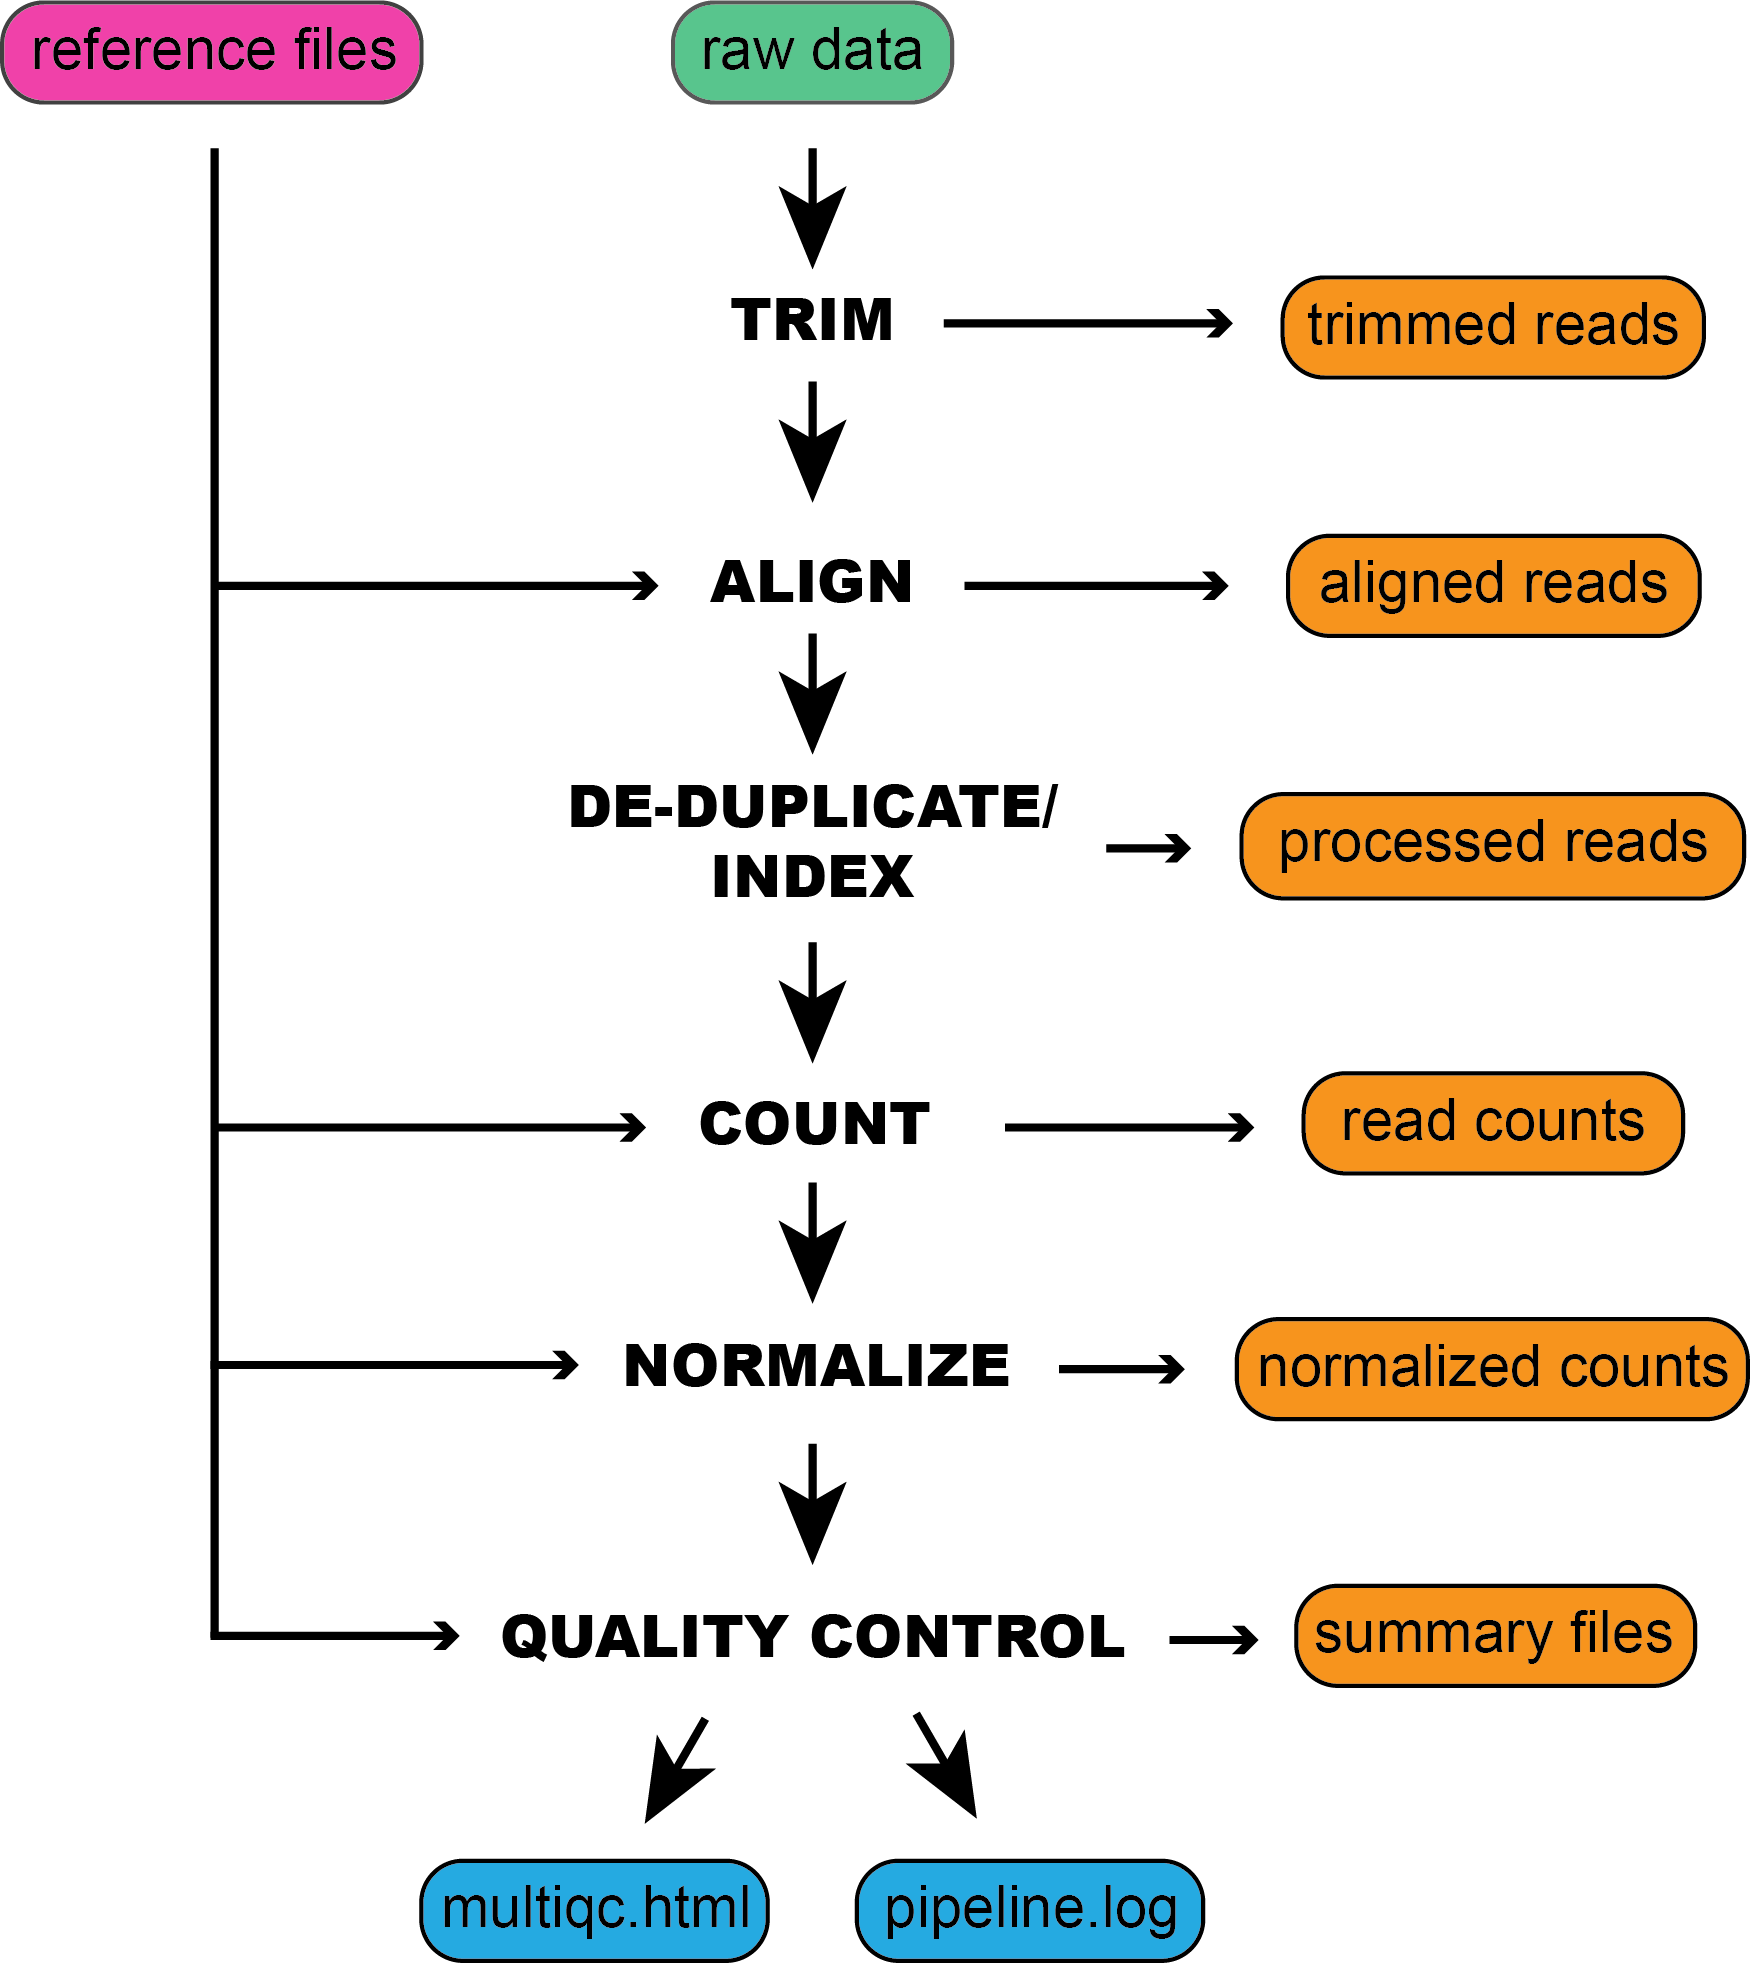
\includegraphics[width=120mm]{figures/xpresspipe_overview.png}
  \caption{An example schematic of the inputs required by XPRESSpipe and organization of the ouputs.}
  \label{fig:outputs}
\end{figure}


\subsection{XPRESSplot}
Further analysis of ribosome profiling or RNA-seq data is handled within XPRESSplot. XPRESSplot is a Pythonic library of analysis and plotting tools that builds upon existing packages, such as Matplotlib \cite{matplotlib} and Seaborn \cite{seaborn} to generate flexible, specific analyses and plots frequently used by biological researchers that can each be executed in a single line of code rather then tens to hundreds. Additionally, many included features are currently available in an R or other programming language package but not in a Python package, a programming language becoming more and more popular in biological research. Brief summaries of key components of this package, as well as descriptions of new or more automated tools is provided below and methods are discussed in subsequent sections. We refer the reader to the documentation (https://xpressplot.readthedocs.io/en/latest/?badge=latest) for more details instructions for other features currently in the toolkit, as well as for future features to be added. While XPRESSplot is designed for handling transcriptomics datasets, is also capable in many cases of handling other omics datasets, such as proteomics or metabolomics.

\subsubsection{Getting Data}
Generally, two inputs are required for all functions within XPRESSplot:

\begin{enumerate}
  \item \textbf{Expression Matrix}: It is assumed the input data matrix = \textit{i} * \textit{j} where \textit{i} (columns) are samples and \textit{j} (rows) are genes or other relative measurement points.
  \item \textbf{Metagene Table}: It is assumed the metagene table is a two column, header-less data matrix where column 0 is the sample ID (as specified in \textit{i} of the expression matrix) and column 1 is the sample group (for example, wild-type or treatment).
\end{enumerate}

\subsubsection{Normalization}
RNA-seq experiments can be normalized using the reads-per-million (RPM), Reads-per-kilobase-million (RPKM) or Fragments-per-kilobase-million (FPKM), and transcripts per million (TPM) methods, as outlined in Equations 1-4 in the Methods \cite{evans_briefbio}. Other normalizations, such as mean centering of \textit{j} features (i.e. genes or other items) by sklearn's preprocessing module \cite{scikit_learn}. Count thresholds can also be set to remove genes from analysis that may be less reliable due to poor ability to be sequenced.

\subsubsection{Analyzing Data}

While a litany of analysis tools are included in XPRESSplot as of the time of writing, we will focus on tools unique to this Python library or particularly useful and refer to reader to the documentation for further details and examples of additional analysis features.

\begin{itemize}
  \item \textbf{Principle Components Analysis}: Principle components analysis (PCA) for the data matrix is computed using Python's scikit-learn package \cite{scikit_learn} and desired principle components are plotted in a scatter plot via the matplotlib \cite{matplotlib} and seaborn \cite{seaborn} packages. The XPRESSplot PCA module, as in many other analysis modules within XPRESSplot, samples are color-coded by cross-referencing the data matrix with the metagene table to determine sample labels. A dictionary is additionally passed into the function that maps a particular color to each sample label. Confidence intervals are plotted over the scatterplot using numpy \cite{numpy1, numpy2}, a feature lacking from Pythonic PCA packages.

  \item \textbf{Volcano Plot}: Volcano plots are an efficient method for plotting magnitude, direction, and significance of changes in expression or other data types between two conditions with multiple replicates each. By providing the categorical names for samples of two conditions in the metadata matrix, XPRESSplot will automate the calculation and plotting of this plotting method. For each gene, expression levels are averaged between the two conditions and the log\textsubscript{2}(fold change) is calculated. Additionally, for each gene, the P-value between the two conditions is calculated using scipy's individual T-test function \cite{scipy}. The log\textsubscript{2}(fold change) and -log\textsubscript{10}(P-value) is then plotted for each gene between the two conditions. Additional features available are the ability to plot threshold lines, highlight subsets of genes within the plot, and label specific genes by name.

  \item \textbf{Differential Expression Analysis}: XPRESSpipe includes a Python wrapper for DESeq2 for performing differential expression analysis of count data. We refer users to the original publication for more information about uses and methodology \cite{deseq2}.

\end{itemize}

\subsection{Validation}
In order to evaluate the ability of XPRESSpipe to provide the user with reliable results, we processed publicly available raw sequence files through the pipeline. We chose to highlight a ribosome profiling dataset and a subset of TCGA samples to showcase the utility of XPRESSpipe for rapidly gleaming interesting molecular patterns and insights from publicly available data.

\subsubsection{Ribosome Profiling Data and New Insights from Old Data}
The integrated stress response (ISR) is a signaling mechanism used by cells and organisms due to a variety of cellular stresses and has been associated with a variety of diseases. Of particular interest, many disorders resulting in neurological decline are associated with the ISR \cite{isr_disease}. While acute ISR is essential for proper cell survival, long periods of sustained ISR can be damaging. A recently discovered molecule, ISRIB, has recently come under the spotlight for its therapeutic potential and relative lack of side-effects. Interestingly, ISRIB is able to suppress low levels of ISR, while seemingly uneffective at managing acute, high-levels of ISR. It has also been shown to be neuroprotective in mouse models of acute neurological damage \cite{isrib_activation, isrib_structure, isrib_riboseq, isrib_neuroprotective}. \par

A recent study (GSE65778) utilized ribosome profiling in order to better understand the mechanisms of ISRIB in the context of ISR, modeled by tunicamycin (Tm) treatment in HEK293T cells \cite{isrib_riboseq}. Some key findings from this study were that during acute ISR, a specific subset of mRNAs were translationally regulated, and that canonical transcription factors were part of this response. In order to showcase the utility of XPRESSpipe in re-analyzing ribosome profiling and sequencing datasets, we re-processed and analyzed this dataset using the more current \textit{in silico} techniques included in the XPRESSpipe package to shed more light on the mechanisms of ISR and ISRIB's mode of action during ISR. Compared to the raw count data made available in the original manuscript, samples showed comparable alignment rates (Spearman R values ranging from 0.83-0.91) (Figure \ref{fig:figure2}A) as, according to the methods of the original paper, a now outdated alignment program, TopHat2 \cite{tophat2}, was used that has a documented higher false positive alignment rate compared to STAR \cite{alignment_benchmark, star}. Processing of replicates within the XPRESSpipe method showed excellent correlation (Spearman R values all \textgreater 0.98) (Figure \ref{fig:figure2}B). Interestingly, de-duplication of ribosome footprint samples appeared to improve the count values correlations, which may be in part due to the inherent bias of certain sequences by CircLigase, used in the creation of these libraries \cite{circligase_bias, isrib_riboseq} (Figure \ref{fig:supplement2}A). Additionally, samples appeared to be relatively comparable to one another once RPM normalization was performed with few outliers (Figure \ref{fig:supplement2}B). \par

\begin{figure}
\centering
  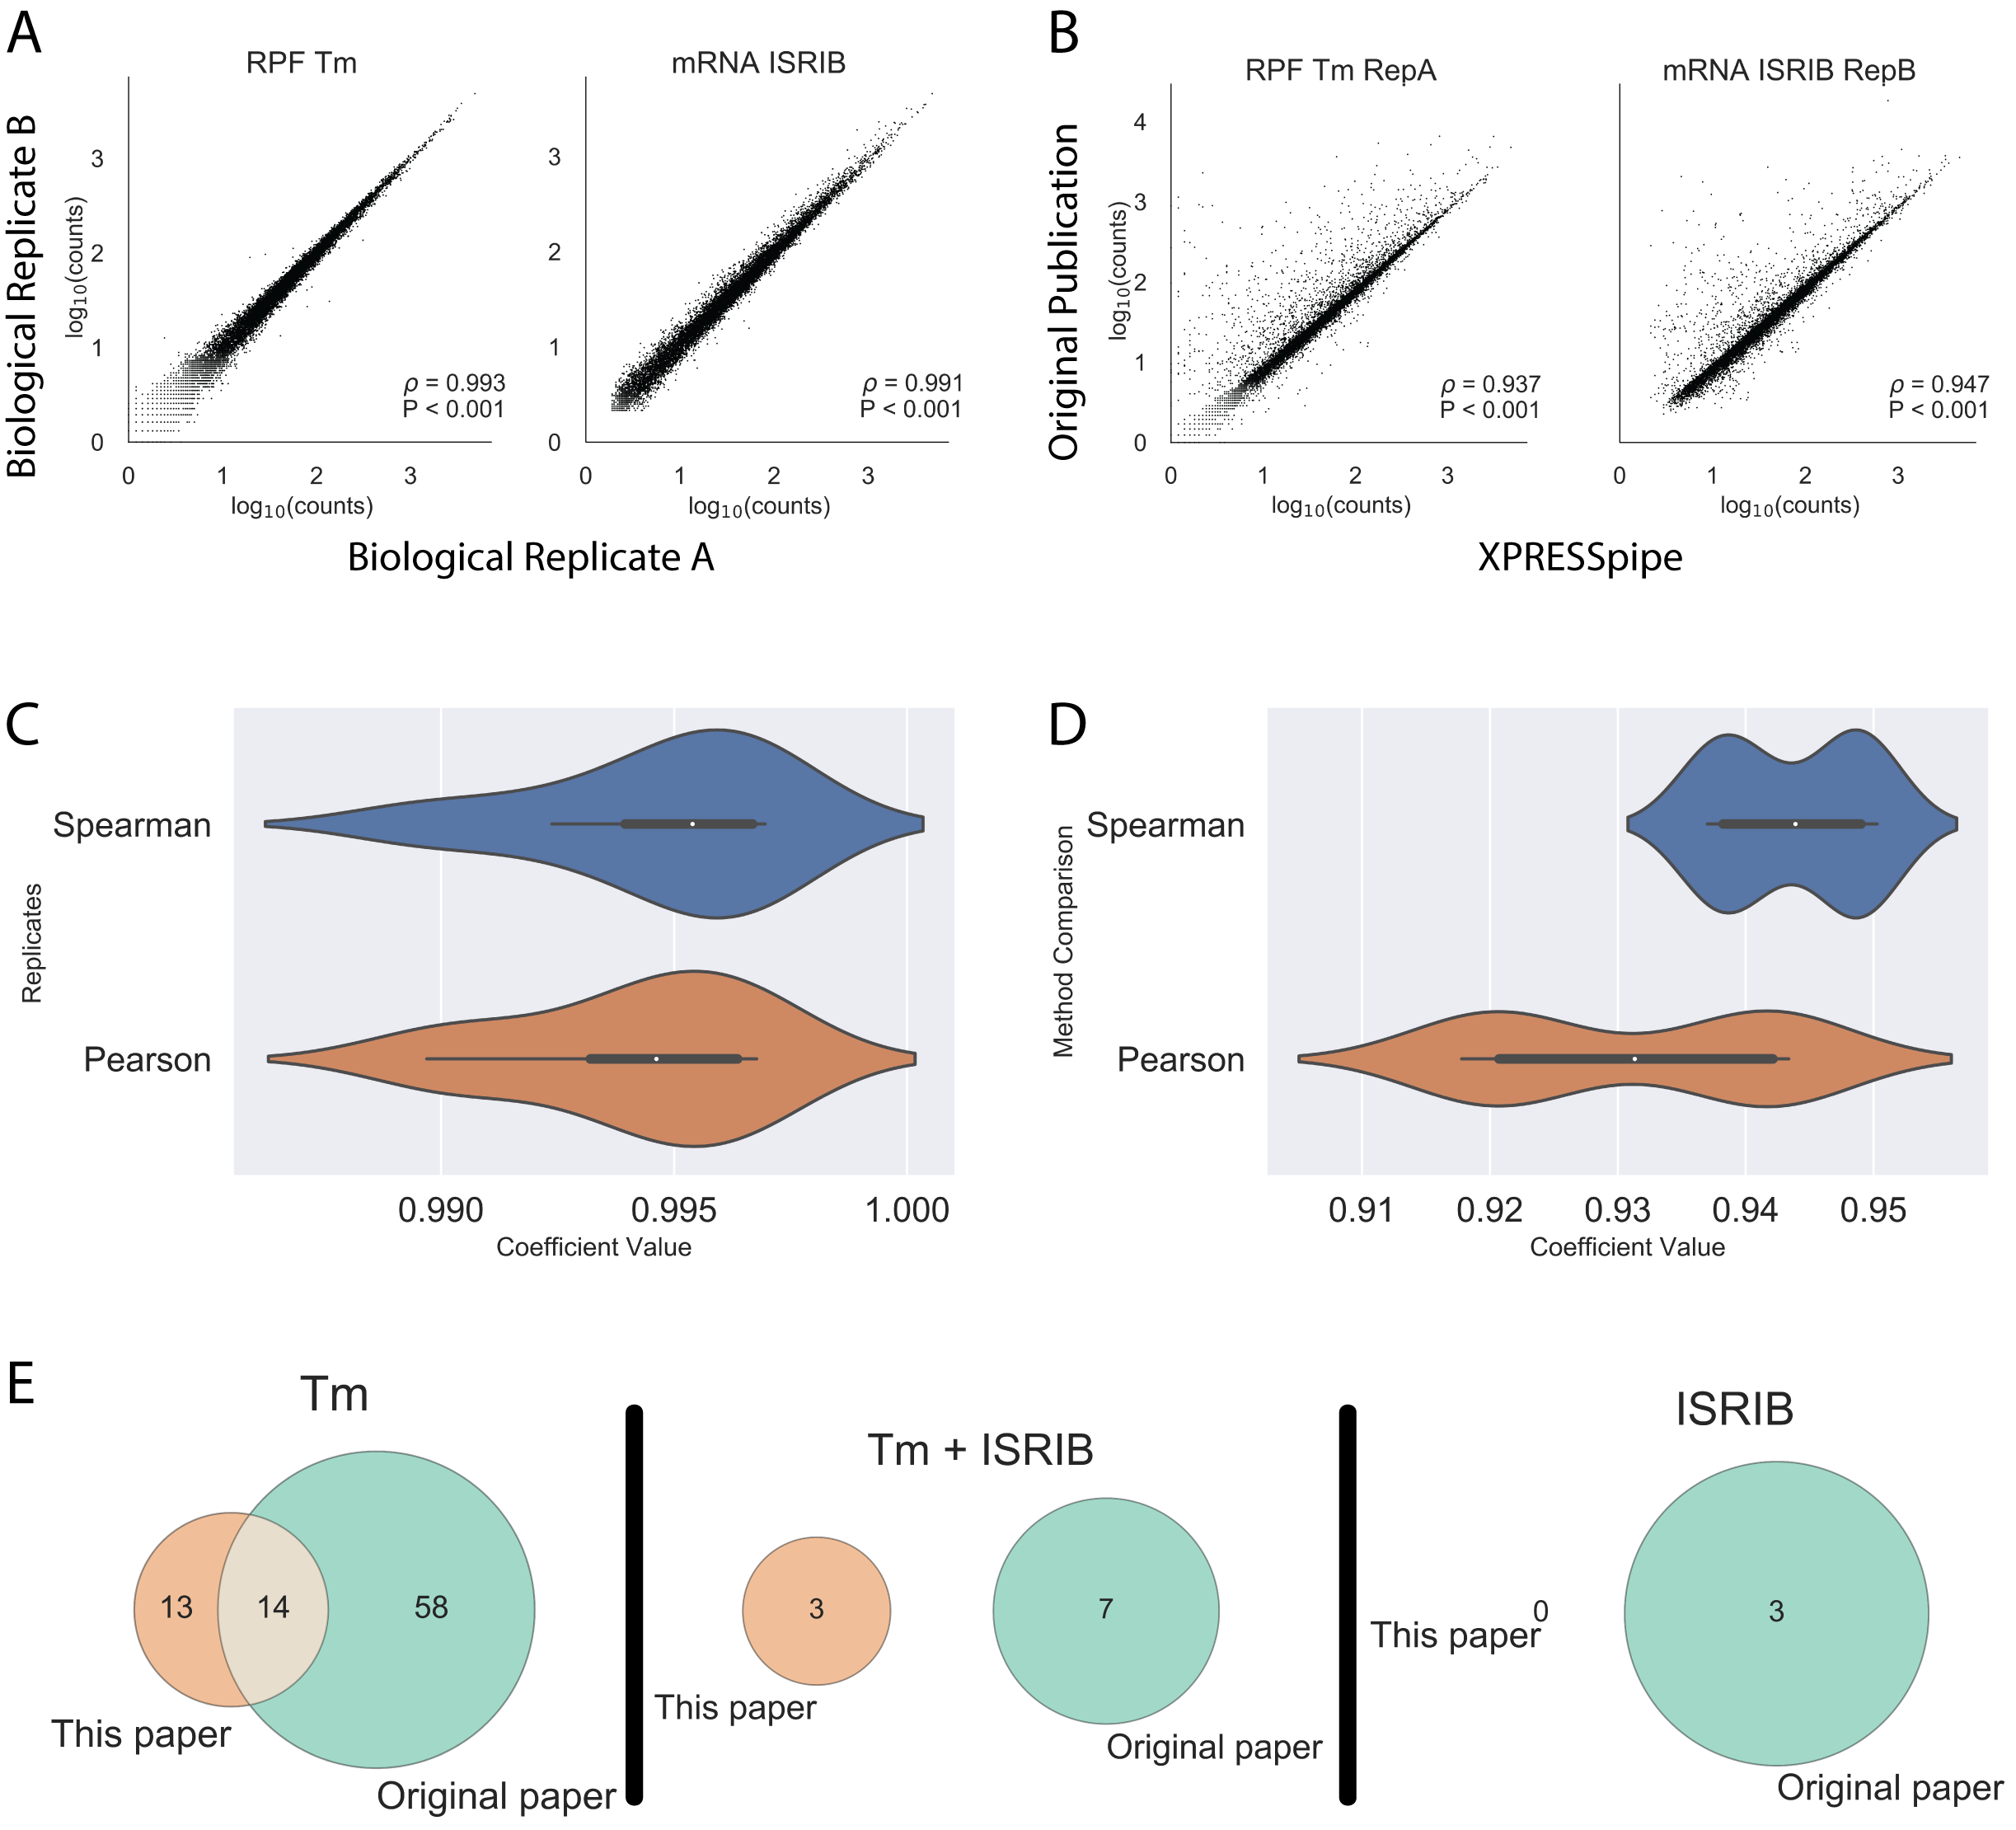
\includegraphics[width=160mm]{figures/xpresspipe_figure2.png}
  \caption{Broad sample quality control and comparision to original processing. A) Cross-processing comparisions between original manuscript and XPRESSpipe. B) Intra-processing comparisions between replicates for XPRESSpipe processing. Note: All R values reported are Spearman R values.}
  \label{fig:figure2}
\end{figure}

XPRESSpipe-processed samples revealed similar canonical targets of translational regulation during ISR were identified as in the original study, such as ATF4, ATF5, and PPP1R15A (Figure \ref{fig:figure3}A, highlighted in magenta) \cite{isrib_riboseq}. Of note, the fold change in translation efficiency of ATF4 (2.027) from XPRESSpipe-processed samples more closely matches the biochemically validated levels of up-regulation under a variety of ISR inducers, where ATF4 translation upregulation generally increased 2-3 fold, with some more extreme cases increasing up to 4 fold \cite{atf4_translation}. Other targets highlighted in the original study \cite{isrib_riboseq}, such as ATF5 and PPP1R15A also increased in their  translation efficiency fold change (2.178 and 2.594, respectively) (Figures \ref{fig:figure3}A, B; \ref{fig:supplement3}A, B).  \par

In the original study, the genes translationally down-regulated appeared to reveal no discernable pattern of regulation related to ISR and ISRIB treatment. However, re-analyzing these data with updated the updated methodology within XPRESSpipe may shed new light on an interesting, potentially relevant subset of genes to the neuroprotective properties of ISRIB. Cross-referencing the XPRESSpipe data with the de-duplicated counts (as discussed above), and intersecting genes with an FDR \textless 0.05 and a ribosome footprint fold change \textless 0.6 in the non-deduplicated dataset and a fold change \textless 0.5 in the duplicated dataset, all genes contain some phenotypic or functional annotation related to cognitive function, as listed in Table \ref{tab:targets} (descriptions sourced from www.genecards.org and www.omim.org). The translational down-regulation of these genes could likely play a role in the cognitive decline associated with ISR and the rescue in translation during ISRIB may partially explain the drugs neuroprotective properties. Further analysis of these potential hits is strengthened by investigating the read pile-ups along these genes in IGV \cite{igv}, where footprint coverage is observed across the transcript for all ribosome profiling samples except the Tm-treated samples (Figures \ref{fig:figure3}C, \ref{fig:supplement3}C, D). This provides further support to this observation as use of CircLigase in the library preparation can bias certain reads' incorporation in sequencing libraries, whereas there appears to be none in these samples \cite{circligase_bias}.

\begin{figure}
\centering
  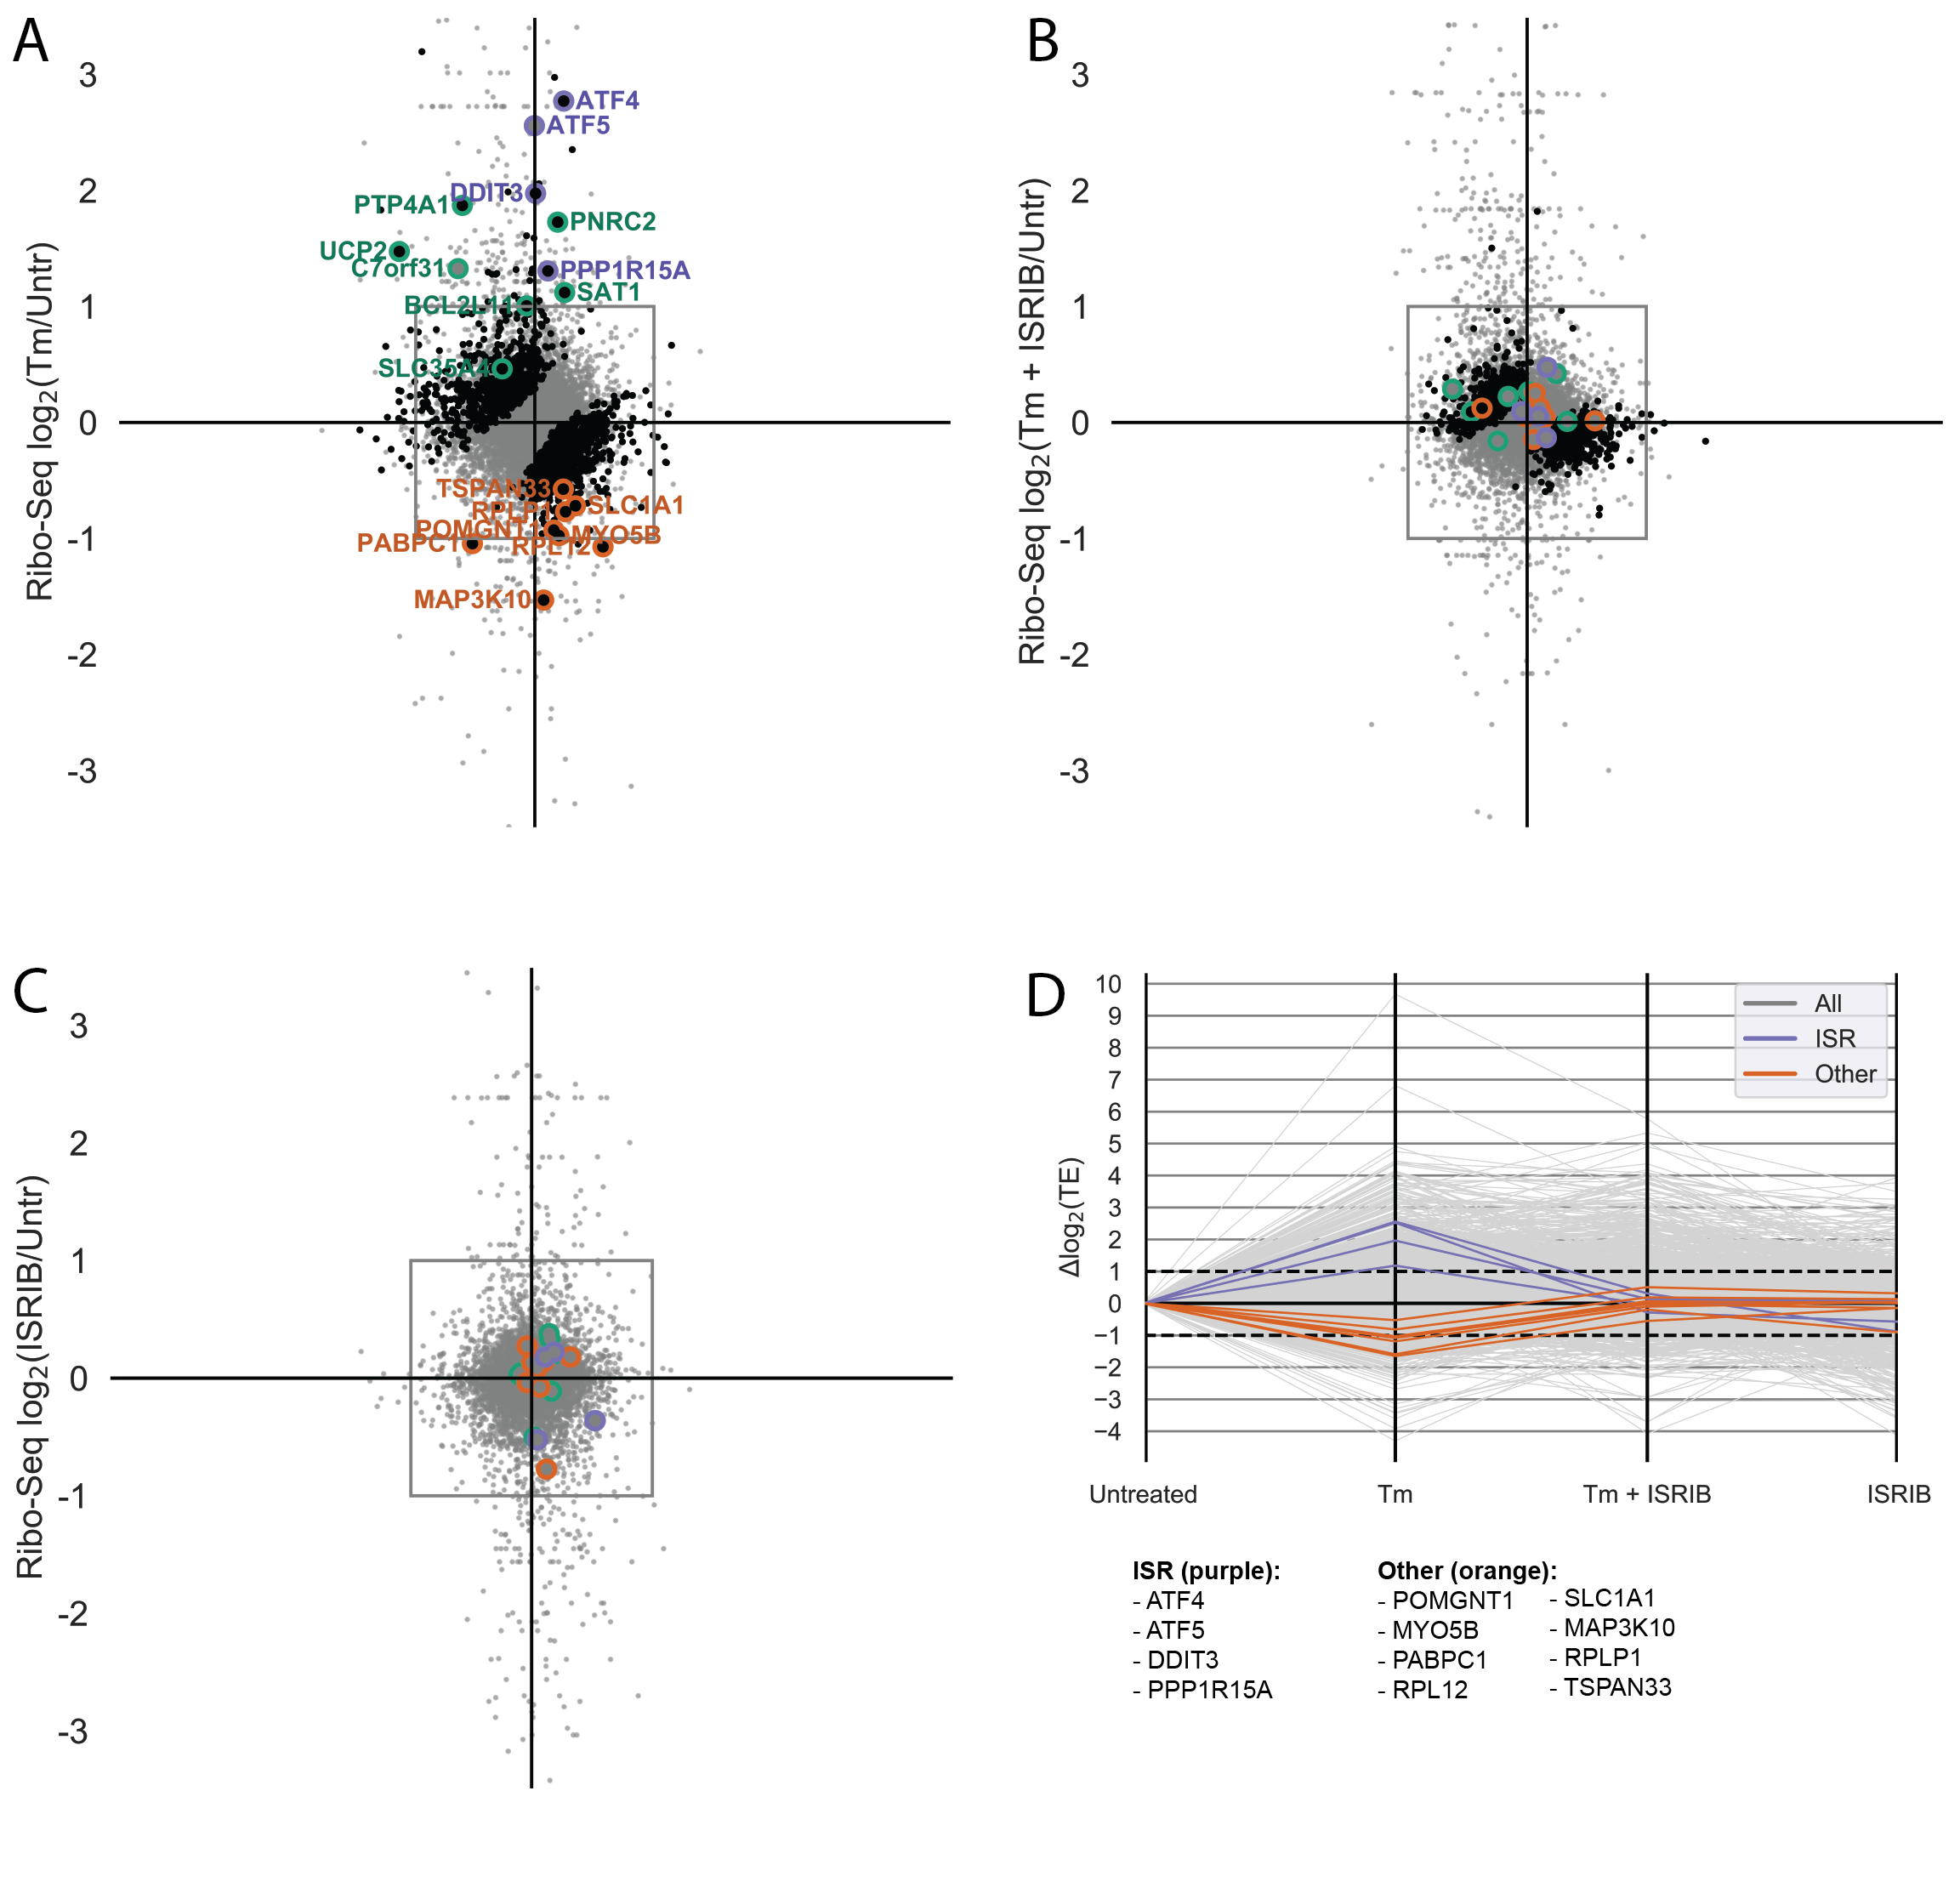
\includegraphics[width=180mm]{figures/xpresspipe_figure3.png}
  \caption{Biological validation and insight into previously published ISR model ribosome profiling data. A) Fold change for each drug condition compared to untreated for the ribosome profiling and RNA-seq data. ISR canonical targets passing fold change and significance threshold during Tm conditions are highlighted in magenta. All translationally down-regulated genes passing fold change and significance threshold during Tm conditions are highlighted in green. B) Changes in log\textsubscript{2} Translation Efficiency compared to Untreated for each drug condition for each of the translationally down-regulated genes passing previous discussed thresholds. C) IGV plot for NOTCH3 for all ribosome profiling samples show read coverage across the transcript.}
  \label{fig:figure3}
\end{figure}

\captionof{table}{Translationally down-regulated genes during acute Tm treatment.}
\begin{tabular}{p{2.5cm}p{15.5cm}}
 \textbf{Gene Name} & \textbf{Relevant Description} \\
 \hline
 MYO5B & Identified in a screen for large proteins expressed in brain; Encodes molecular motor that utilizes energy from ATP hydrolysis to generate mechanical force, required for the recycling of transferrin receptor back to the plasma membrane through an endocytotic recycling compartment in nonpolarized cells. \\
 \hline
 NOTCH3 & Establishes an intercellular signalling pathway that plays a key role in neural development; Mutations in NOTCH3 have been identified as the underlying cause of cerebral autosomal dominant arteriopathy with subcortical infarcts and leukoencephalopathy \\
 \hline
 NGEF & Overexpressed in brain; Involved in axon guidance regulating ephrin-induced growth cone collapse and dendritic spine morphogenesis \\
 \hline
 POMGNT1 & Mutations in this gene may be associated with muscle-eye-brain disease and several congenital muscular dystrophies \\
 \hline
 ENPP5 & Suggested role in neuronal cell communications in rat studies \\
 \hline
 CCNG2 & Overexpressed in brain; Tightly regulated in cell cycle \\
 \hline
 SMURF2 & Interacts with SMAD proteins; Functions in regulation of neuronal and planar cell polarity, induction of senescence, and tumor suppression \\
 \hline
 ARHGEF6 & Mutations cause X-chromosomal non-specific cognitive disability and other neurodevelopmental abnormalities \\
 \hline
 FGFRL1 & Highly expressed in brain; Sets in motion a cascade of downstream signals ultimately influencing mitogenesis and differentiation; Behavioral and neurological phenotypes \\
 \label{tab:targets}
\end{tabular}
\newline

\subsubsection{Performance Validation Using TCGA Data}
\textit{In this section, we will process the raw data for 10-20 TCGA samples and compare the FPKM counts output by XPRESSpipe to the publicly available FPKM counts for the relevant samples.
This will a simple section with one supplemental figure showing comparisons and probably end up being added right before bioRXiv submission.
Summarize metrics (total reads mapped, etc)
PE application sent to CHPC, waiting for project space set-up}

\subsubsection{Cost Analysis}
XPRESSpipe functions can be computationally intensive and thus super-computing resources are recommended. Many universities provide super-computing resources to their staff; however, in cases where these resources are not available, servers such as Amazon Web Services (AWS) (https://aws.amazon.com/) can be used to process sequencing data using XPRESSpipe. For example, the ribosome profiling dataset of 32 raw sequence files used in the study was processed using the University of Utah's Center for High Performance Computing resources. Run statistics can be found in Table \ref{tab:chpc_performance}.

% UPDATE BEFORE SUBMISSION ONCE QUALITY CONTROL STABLE AND CHECK CONVERSIONS
\captionof{table}{XPRESSpipe processing statistics for dataset GSE65778.}
\begin{tabular}{p{5cm}p{3cm}}
\textbf{Metric} & \textbf{Value} \\
\hline
 Elapsed Real Time & 07h39m47s \\
 \hline
 Total CPU Time & 1d04h34m36s  \\
 \hline
 Allocated CPUs & 16 \\
 \hline
 Allocated Memory per Node & 62.50GB \\
 \hline
 Maximum RAM of all tasks & 62.79GB \\
 \label{tab:chpc_performance}
\end{tabular}
\newline

Based on these metrics, if HPC services weren't locally available for a user, one could use Amazon Web Services to process the data for relatively little money. For a comparable run, storage cost would amount to around 14 USD on Amazon S3 storage and compute cost for a similar computational node for the given elapsed time would cost around 6 USD using Amazon EC2 On-Demand (however, significantly reduced rates are available if using Spot instances).


\subsubsection{Comparisons to Other Workflows}
\textit{I'm not sure quite sure how to handle a benchmarking with this as RiboGalaxy it very different and is not directly comparable -- is the TCGA and ISRIB validation enough?}


\section{Discussion}
We have described herein a new software suite, XPRESSyourself, a collection of tools to aid in expression data processing and analysis. While RNA-seq technologies are becoming more and more mature, standardized protocols are lacking. This is problematic when individuals or groups may not be using the most up-to-date methods or be aware of particular biases or measures of quality control required to produce a reliable, high-quality sequencing study. XPRESSpipe handles these issues for the user by continuously updating to utilize the best-performing software tools in sequencing as measured by peer-reviewed benchmarking studies. It also outputs all necessary quality control metrics so that the user can quickly assess quality and identify any systematic problems or technical biases that may be present in their samples. \par

An additional problem XPRESSpipe addresses is use these software tools properly, especially for those coming from a non-computational background. This is especially important in situations where a bioinformatics core may be so backlogged it takes 2-4 months to process a dataset, which is inhibitory to scientific discovery and dissemination. XPRESSyourself will dissolve this barrier to entry for most users so that they can process and analyze their data immediately upon receipt of the raw data and only requires simple programming knowledge covered by a variety of free online programs (such as https://www.codecademy.com/learn/learn-the-command-line). These users can also be assured they are using the most up-to-date standard for RNA-seq processing and analysis. \par

Tools previously missing from the general ribosome profiling toolkit have also been added within XPRESSyourself. This includes GTF truncation of transcripts in a recursive manner over exon space and rRNA probe design aids for removing contaminating rRNA sequences in ribosome profiling libraries that are difficult to remove with commercial kits. \par

We demonstrated the utility of the XPRESSyourself toolkit by re-analyzing a publicly available ribosome profiling dataset. From this analysis, we identified putative hits that may contribute to the neurodegenerative effects of integrated stress response (ISR) and how the molecule ISRIB may be acting on these hits to act as a neuroprotective agent. This additionally highlights the importance of re-analyzing older datasets with more current methods, as over time methodologies improve to reduce errors. We also showed the capability of quickly processing data on TCGA data. These principles are transferable to new datasets and XPRESSyourself will have individuals and labs take sequence processing and analysis into their own hands to avoid long queues with bioinformatics cores, save money, and generally democratize the process. \par

While XPRESSyourself's pipeline may be somewhat more time and computationally intensive than other pipelines, the trade-off is higher quality alignments and quantification, and unless analyzing thousands of samples, is generally not too expensive or time-consuming.


\section{Conclusions}
With the adoption of this pipeline, the field of high-throughput sequencing can begin to arrive towards a standardized processing protocol for sequencing data and eliminate some of the variability that comes from using a variety of software packages for various steps during read processing. XPRESSpipe will act as a flexible pipeline that will be updated with the best performing packages as future tools are created and benchmarks performed. Additionally, various tools missing from the ribosome profiling and RNA-seq communities have been added as part of this pipeline. With these tools, such as the GTF modification sub-module, genome reference formatting and curation is automated and accessible to the public. Further, by using this pipeline on publicly available data, we highlight XPRESSpipe's utility in being able to re-process publicly available data or personal data to uncover novel biological patterns quickly. Adoption of this tool will aid the average scientist is quickly accessing their data, using the highest-quality methods.


\section{Materials and Methods}

\subsection{Software Dependencies}
A list of dependencies required for XPRESSpipe is listed in Table \ref{Tab:software_pipe}. Dependencies for XPRESSplot are listed in Table \ref{Tab:software_plot}.

% Software dependencies table
\captionof{table}{Summary of dependency software, accession location, and purpose in the XPRESSpipe package.}
\begin{tabular}{p{2.4cm}p{7.5cm}p{3cm}}
 \textbf{Package} & \textbf{Purpose} & \textbf{Reference} \\
 \hline
 Python & Primary language & \\
 \hline
 R & Language used for some statistical modules & \\
 \hline
 fastp & Read pre-processing & \cite{fastp} \\
 \hline
 STAR & Reference curation and read alignment & \cite{star} \\
 \hline
 samtools & Alignment file manipulation & \cite{samtools} \\
 \hline
 bedtools & Alignment file manipulation & \cite{bedtools} \\
 \hline
 deepTools & Alignment file manipulation & \cite{deeptools} \\
 \hline
 Cufflinks & Read quantification (primary) & \cite{cufflinks} \\
 \hline
 HTSeq & Read quantification & \cite{htseq} \\
 \hline
 FastQC & Quality Control & \cite{fastqc} \\
 \hline
 MultiQC & Quality Control & \cite{multiqc} \\
 \hline
 dupRadar & Measure library complexity & \cite{dupradar} \\
 \hline
 pandas & Data manipulation & \cite{pandas} \\
 \hline
 numpy & Data manipulation & \cite{numpy1, numpy2} \\
 \hline
 scipy & Data manipulation & \cite{scipy} \\
 \hline
 sklearn & Data manipulation & \cite{sklearn} \\
 \hline
 matplotlib & Plotting & \cite{matplotlib} \\
 \hline
 XPRESSplot & Normalization and matrix manipulation & This paper \\
 \hline
 rsubread & Dependency for dupRadar &  \\
 \hline
 dupRadar & Perform library complexity calculations & \cite{dupradar} \\
 \hline
 deseq2 & Perform differential expression analysis & \cite{deseq2} \\
 \label{Tab:software_pipe}
\end{tabular}
\newline

% Software dependencies table
\captionof{table}{Summary of dependency software, accession location, and purpose in the XPRESSplot package.}
\begin{tabular}{p{2.4cm}p{7.5cm}p{3cm}}
 \textbf{Package} & \textbf{Purpose} & \textbf{Reference} \\
 \hline
 Python & Primary language & \\
 \hline
 R & Language used for some statistical modules & \\
 \hline
 pandas & Data manipulation & \cite{pandas} \\
 \hline
 numpy & Data manipulation & \cite{numpy1, numpy2} \\
 \hline
 scipy & Data manipulation & \cite{scipy} \\
 \hline
 matplotlib & Plotting & \cite{matplotlib} \\
 \hline
 seaborn & Plotting & \cite{seaborn} \\
 \hline
 plotly & Plotting & \cite{plotly} \\
 \hline
 sklearn & Data manipulation & \cite{sklearn} \\
 \hline
 GEOparse & Access GEO data & \cite{geoparse} \\
 \hline
 DESeq2 & Perform differential expression analysis & \cite{deseq2} \\
 \hline
 sva & Perform batch correction for known effects with the ComBat function & \cite{sva} \\
 \label{Tab:software_plot}
 \end{tabular}
 \newline

\subsection{GTF Modification}
Protein coding genes are identified by the ``protein\_coding" annotation within \texttt{attribute} column of the GTF file.
Longest transcripts are determined by calculating the exon space for each transcript associated with a given \texttt{gene\_id}. If a pre-mature stop is annotated within a transcript, that is considered the end-point of the transcript length. \par
Truncation is performed by identifying the 5' and 3' end of each transcript and modifying the given coordinates to reflect the given truncation amounts. The amounts to be truncated can be modulated by the user; however, suggested ranges are 45 nt from the 5' end and 15 nt from the 3' end, set as the default parameters for the function \cite{ingolia_meth}. As a given exon may be less than the specified amounts, the function will recursively search exon by exon until the full truncated amount is trimmed.

\subsection{Normalization}
Equations 1-4 reflect the design of the normalization functions within XPRESSplot.

  \begin{equation}
    RPM = \frac{(\#\ number\ reads\ per\ gene)\ \cdot\ 1e6}{(\#\ mapped\ reads\ per\ sample)}
  \end{equation}
  \begin{equation}
    RPKM = \frac{(\#\ number\ reads\ per\ gene)\ \cdot\ 1e6\ \cdot\ 1e3}{((\#\ mapped\ reads\ per\ sample)\ \cdot\ (gene\ length\ (bp))}
  \end{equation}
  \begin{equation}
    FPKM = \frac{(\#\ number\ fragments\ per\ gene)\ \cdot\ 1e6\ \cdot\ 1e3}{(\#\ mapped\ fragments\ per\ sample)\ \cdot\ (gene\ length\ (bp))}
  \end{equation}
  \begin{equation}
    TPM = \frac{(\#\ number\ fragments\ per\ gene)\ \cdot\ 1e3\ \cdot\ 1e6}{(gene\ length\ (bp))\ \cdot\ (\#\ mapped\ fragments\ per\ sample)}
  \end{equation}

\subsection{Quality Control Summary Plotting}
Summary plots are created using pandas \cite{pandas} and matplotlib \cite{matplotlib}. Kernel density plots for library complexity analyses are created using numpy \cite{numpy1, numpy2} and scipy's \texttt{gaussian\_kde} function \cite{scipy}.

\subsection{Metagene Estimation}
Metagene calculations are performed by determining the meta-genomic coordinate \textit{M} for each aligned read, where \textit{L\textsubscript{e}} is the leftmost coordinate of the mapped read and \textit{r} is the length of the mapped read. \textit{S} denotes the start coordinate for the transcript and \textit{l\textsubscript{e}} is the cumulative length of all exons for the given transcript. The subscripted \textit{e} indicates the coordinate is relative to exon space, where intron space is not counting in the coordinate relative to the start of the transcript. Required inputs are an indexed BAM file and an unmodified GTF reference file. For each mapped coordinate, the metagene position is calculated as:
\begin{equation}
\textit{M} = \frac{|(L\textsubscript{e}\ +\ \frac{1}{2}r)\ -\ S|\ \cdot\ 100}{\textit{l\textsubscript{e}}}
\end{equation}

In the case where a mapped coordinate falls within multiple genes, a penalty is assigned as:
\begin{equation}
  \textit{c} = \frac{1}{\textit{n}}
\end{equation}
Where \textit{c} is the count score for a given meta-position and \textit{n} is the number of different transcripts a given coordinate mapped. To be counted or factored into the penalty, the meta-position coordinate must fall within exon space.

\subsection{Periodicity}
\textit{p} is the distance from the start coordinate, \textit{L\textsubscript{e}} is the leftmost coordinate of the mapped read, \textit{r} is the length of the mapped read, and \textit{S} denotes the start coordinate for the transcript. The superscript signs associated with \textit{p} indicate strandedness and the subscript \textit{e} indicates the coordinate is relative to exon space. Only reads 28-30 nucleotides long are considered in this analysis. The penalty is calculated in the same manner as in the \texttt{metagene} sub-module.
\begin{equation}
  \textit{p}\textsuperscript{+} = (\textit{L}\textsubscript{e}\ +\ \textit{r} - 16)\ -\ \textit{S}
\end{equation}
\begin{equation}
  \textit{p}\textsuperscript{-} = \textit{S}\ -\ (\textit{L}\textsubscript{e}\ +\ 16)
\end{equation}

\subsection{rRNA Probe}
\texttt{rrnaProbe} works on a directory containing fastqc \cite{fastqc} zip compressed files to detect over-represented sequences for each sample. These sequences are then collated to create consensus fragments. One caveat is that FASTQC collates on exact matching sequences, but these sequences may be 1 nt steps from each other and a single rRNA probe could be used to effectively pull out all these sequences. In order to handle this situation, XPRESSpipe will combine these near matches. A rank ordered list of over-represented fragments within the appropriate length range to target for depletion is then output. A BLAST \cite{blast} search on consensus sequences intended for probe useage can then be performed to verify the fragment maps to an rRNA sequence and is thus a suitable depletion probe.

\subsection{Confidence Interval Plotting}
Confidence intervals within PCA scatterplots generated by XRESSplot are calculated as follows:

\begin{enumerate}
  \item Compute the covariance of the two principle component arrays, \textit{x} and \textit{y} using the numpy.cov() function.

  \item Compute the eigenvalues and normalized eigenvectors of the covariance matrix using the numpy.linalg.eig() function.

  \item Compute the $\theta$ of the normalized eigenvectors using the numpy.arctan2() function and converting the output from radians to degrees using numpy.deg().

  \item Compute the $\lambda$ of the eigenvalues by taking the square root of the eigenvalues.

  \item Plot the confidence intervals over the scatter plot: The center point of the confidence interval is determined from the means of the \textit{x} and \textit{y} arrays. The angle is set equal to $\theta$. The width of the condfidence interval is calculated by
  \[
  \textit{w} = \lambda _{\textit{\scriptsize{x}}}\ \cdot\ \textit{ci}\ \cdot\ 2
  \]
  where \textit{ci} is equal to the corresponding confidence level (i.e. 68\% = 1, 95\% = 2, 99\% = 3). The heighth is similarly computed by
  \[
  \textit{h} = \lambda _{\textit{\scriptsize{y}}}\ \cdot\ \textit{ci}\ \cdot\ 2
  \]
\end{enumerate}

\subsection{Ribosome Profiling Example Data Analysis}
The following xpresspipe command was run to process the raw data, available from GEO. Reference files were taken from Ensembl Human build GRCh38.p12.

\begin{lstlisting}[language=bash, caption=Ribosome profiling processing command.]
# Generate reference files
$ xpresspipe curateReference -o $SCRDIR/references/human_reference -f $SCRDIR/references/human_reference -g $SCRDIR/references/human_reference/transcripts.gtf --sjdbOverhang 49 -l -p -t
# Execute pipeline
$ xpresspipe riboseq -i $SCRDIR/input -o $SCRDIR/output -r $REF --gtf $REF/transcripts_LCT.gtf -e isrib_riboprof -a CTGTAGGCACCATCAAT --method RPKM --sjdbOverhang 49
\end{lstlisting}

Only gene names in common between the original data file and XPRESSpipe output were used for the method comparisons. Genes included in all studies were required to have at least 25 counts across samples to be included in the analysis. Correlations and p-values were calculated using the \texttt{scipy.stats.spearman()} function \cite{spearman_rnaseq}. Sample count distributions were plotted using Seaborn where density is indicated by width of plot and boxplot designating interquartile range are plotted \cite{seaborn}. Fold change and translation efficiency plots were created using matplotlib \cite{matplotlib} and pandas \cite{pandas}. Replicates were combined to calculate fold change values and significance between library groups (condition and library type) was calculated using a Benjamini-Hochberg FDR method from \texttt{statsmodels.stats.multitest()} \cite{statsmodels}. Gene coverage profiles were generating using IGV \cite{igv}. Figures and analyses can be reproduced using the associated scripts found at https://github.com/XPRESSyourself/manuscript (DOI: XXXXXX). \par

Translation efficiency was calculated as follows:

\begin{equation}
  \Delta TE = \frac{RPF\textsubscript{\textit{treatment}}}{mRNA\textsubscript{\textit{treatment}}} - \frac{RPF\textsubscript{\textit{untreated}}}{mRNA\textsubscript{\textit{untreated}}}
\end{equation}

\subsection{Cost Analysis}
Cost analysis was performed by accessing run logs from the HPC and using published AWS prices (https://aws.amazon.com/ec2/pricing/on-demand/, https://aws.amazon.com/s3/pricing/, accessed 28 May 2019) to calculate relative cost for a similar run.

\section*{List of abbreviations}
UMI - unique molecular identifier, nt - nucleotide,

\section*{Ethics approval and consent to participate}
Protected TCGA data were obtained through dbGaP project number 21674 and utilized according to the associated policies and guidelines.

\section*{Consent for publication}
Protected TCGA data were obtained through dbGaP project number 21674 and utilized according to the associated policies and guidelines.

\section*{Availability of data and materials}
The source code for these packages will be perpetually open source and protected under the GPL-3.0 license. The code can be publicly accessed and installed from https://github.com/XPRESSyourself. Updates to the software are version controlled and maintained on GitHub. Jupyter notebooks and video walkthroughs are included on https://github.com/XPRESSyourself for guiding a user through use of the packages. Documentation is hosted on readthedocs \cite{readthedocs} at https://xpresspipe.readthedocs.io/en/latest/ and https://xpressplot.readthedocs.io/en/latest/. The publicly available ribosome profiling data are accessible through GEO series accession number GSE65778. TCGA data are accessible through dbGaP accession number phs000178. Code used to create manuscript figures and analyses can be found at https://github.com/XPRESSyourself/manuscript (DOI: XXXXXX).

\section*{Competing interests}
The authors declare that they have no competing interests.

\section*{Funding}
J.A.B. received support from the National Institute of Diabetes and Digestive and Kidney Diseases (NIDDK) Inter-disciplinary Training Grant T32 Program in Computational Approaches to Diabetes and Metabolism Research, 1T32DK11096601 to Wendy W. Chapman and Simon J. Fisher.

\section*{Contributions}
J.A.B. conceptualized and administered the project; performed all investigation, analysis, visualization, and data curation; provisioned computing resources; acquired funding; amd write the original draft for this study. J.A.B. wrote the software and J.R.B. designed and wrote the rRNA Probe sub-module. J.A.B., J.T.M., A.J.B., and Y.O. performed software and documentation validation. J.A.B., J.R.B., M.T.H., and J.G. and developed the methodology. J.P.R, M.T.H., J.G., and A.R.Q. supervised the study. All authors were involved in reviewing and editing the manuscript.

\section*{Acknowledgments}
The authors wish to thank Mark Wadsworth, Ryan Miller, and Michael Cormier for helpful discussions on pipeline design. They also wish to thank Cameron Waller for helpful discussions related to pipeline design and analysis. The support and resources from the Center for High Performance Computing at the University of Utah are gratefully acknowledged. The computational resources used were partially funded by the NIH Shared Instrumentation Grant 1S10OD021644-01A1.


\bibliography{manubib}
\bibliographystyle{Science}

\beginsupplement
\begin{figure}
\centering
  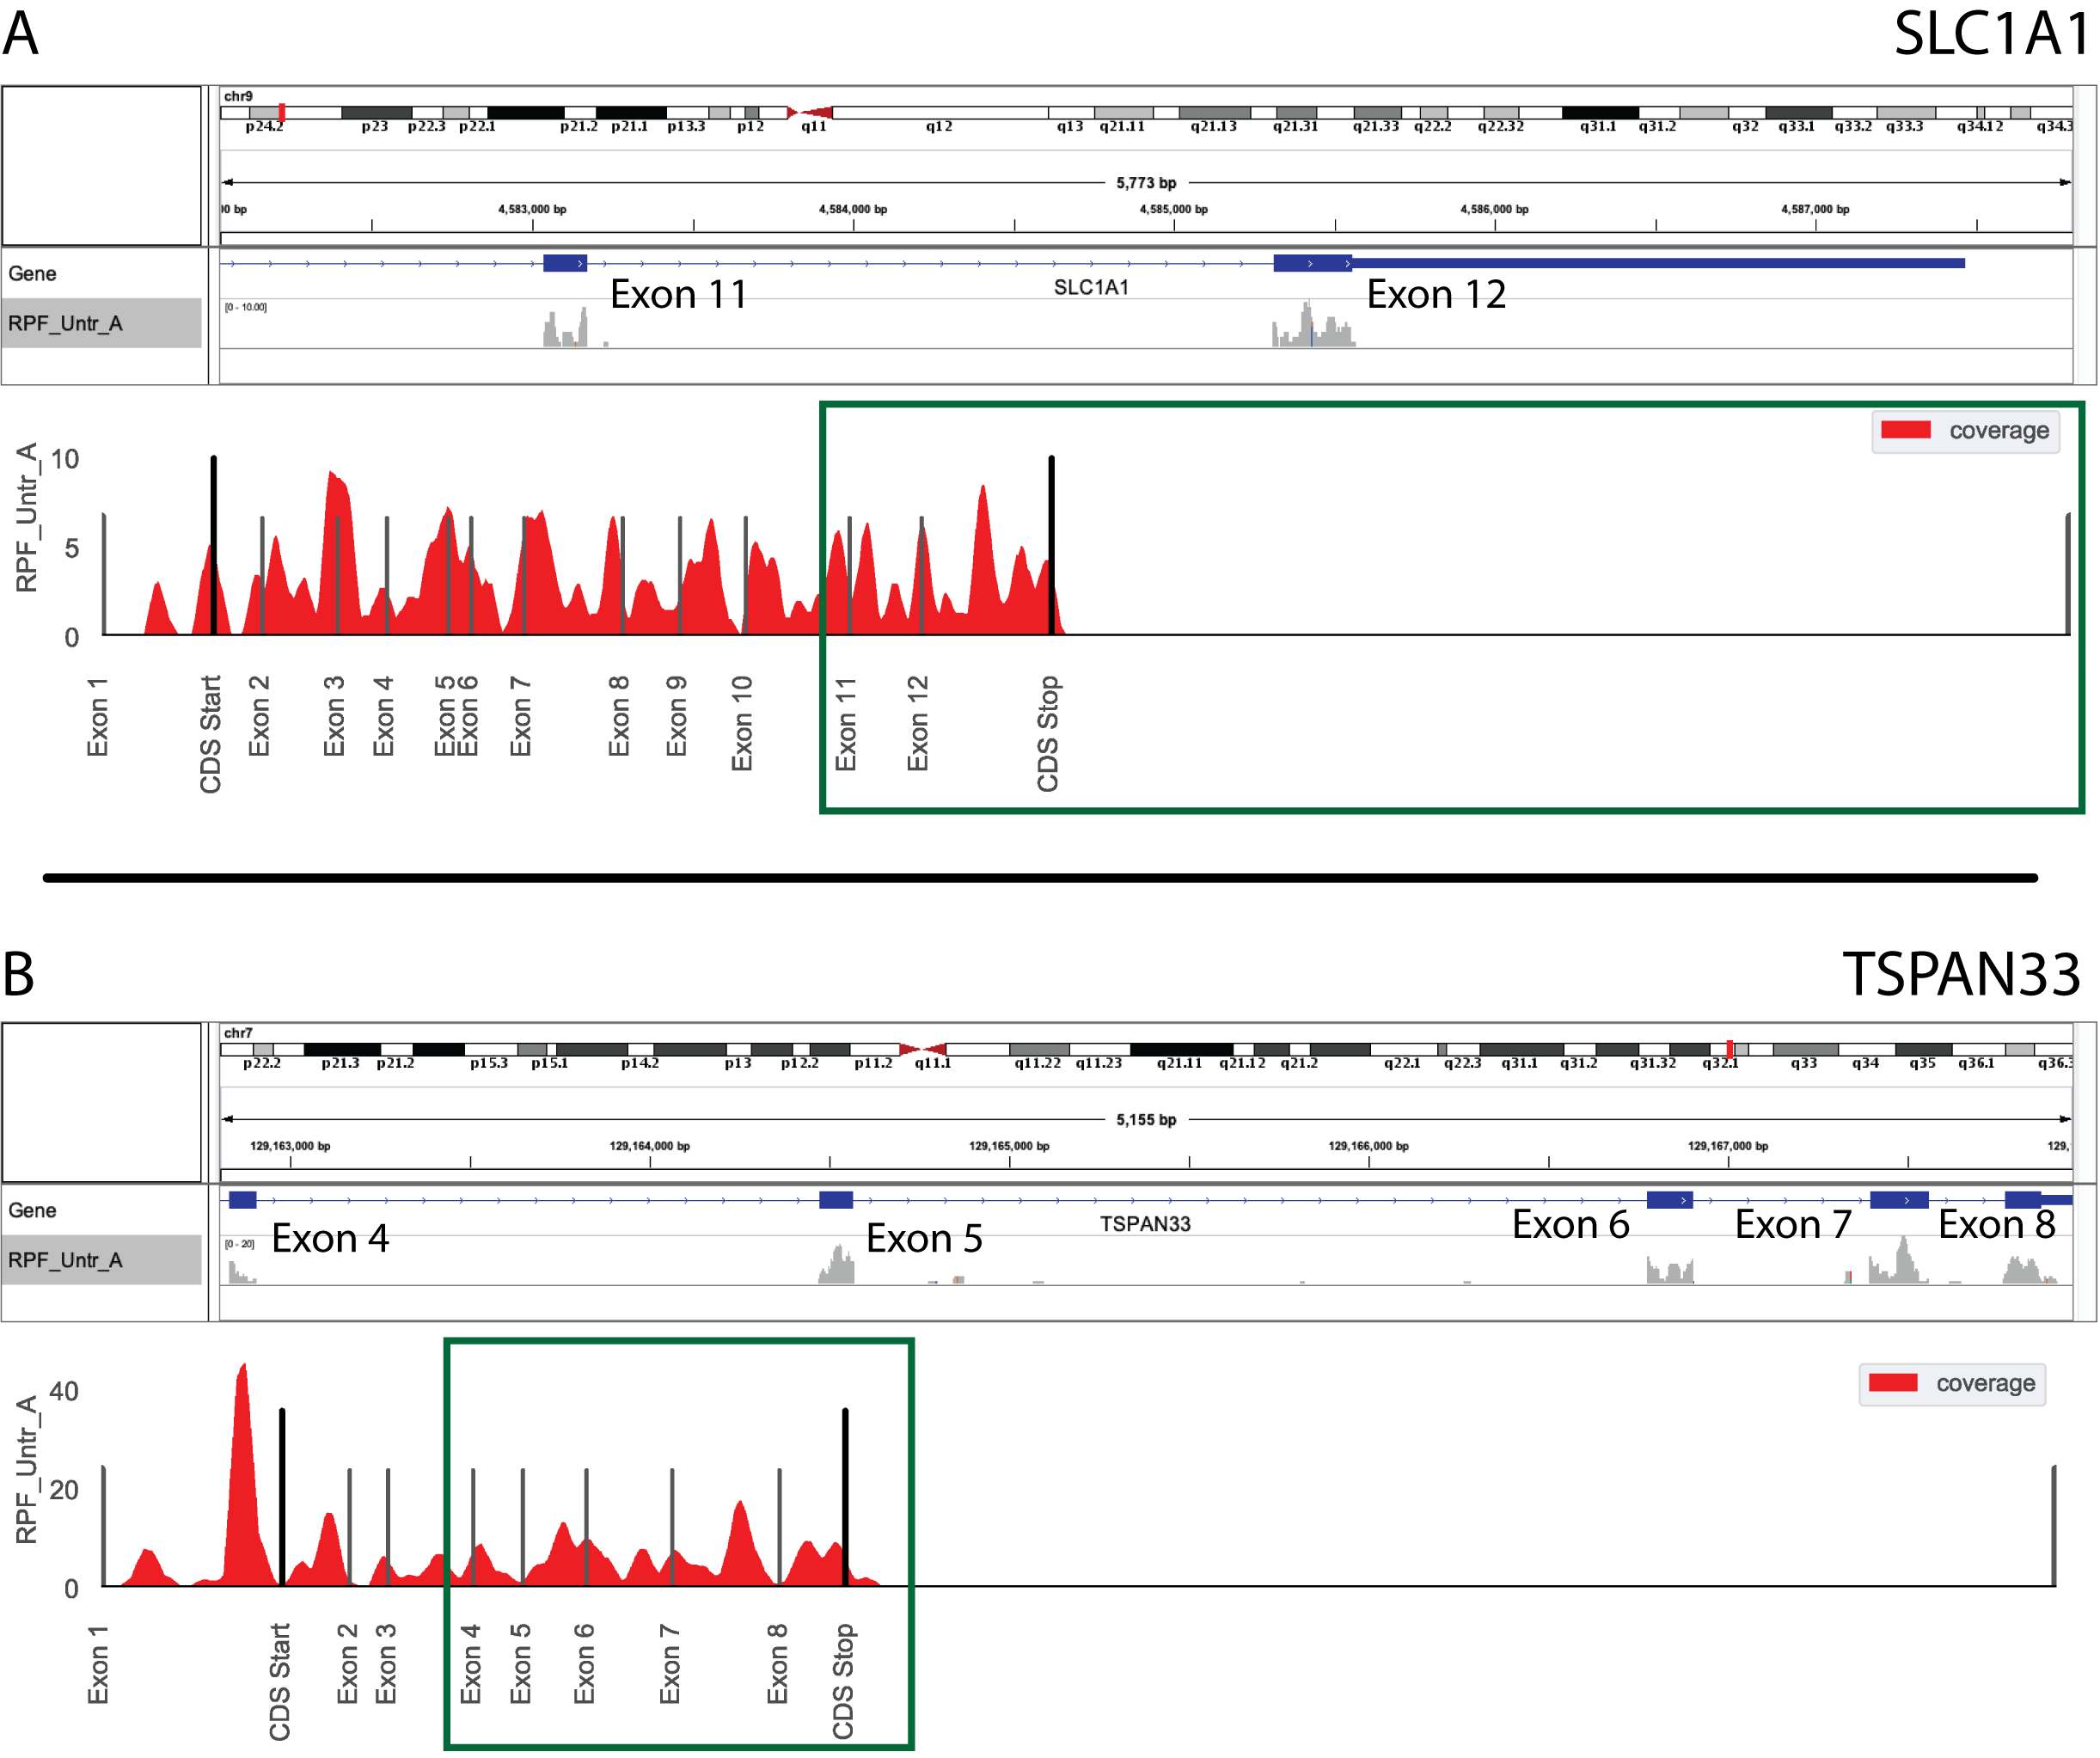
\includegraphics[width=160mm]{figures/xpresspipe_supplement2.png}
  \caption{A) Dispersion of read counts between samples decreases with \textit{in silico} de-duplication. Note: All R values reported are Spearman R values. B) log\textsubscript{10}(RPM) value distributions for XPRESSpipe processed samples. Boxplots embedded within violinplot designate the interquartile range and violinplot reports count density.}
  \label{fig:supplement2}
\end{figure}

\begin{figure}
\centering
  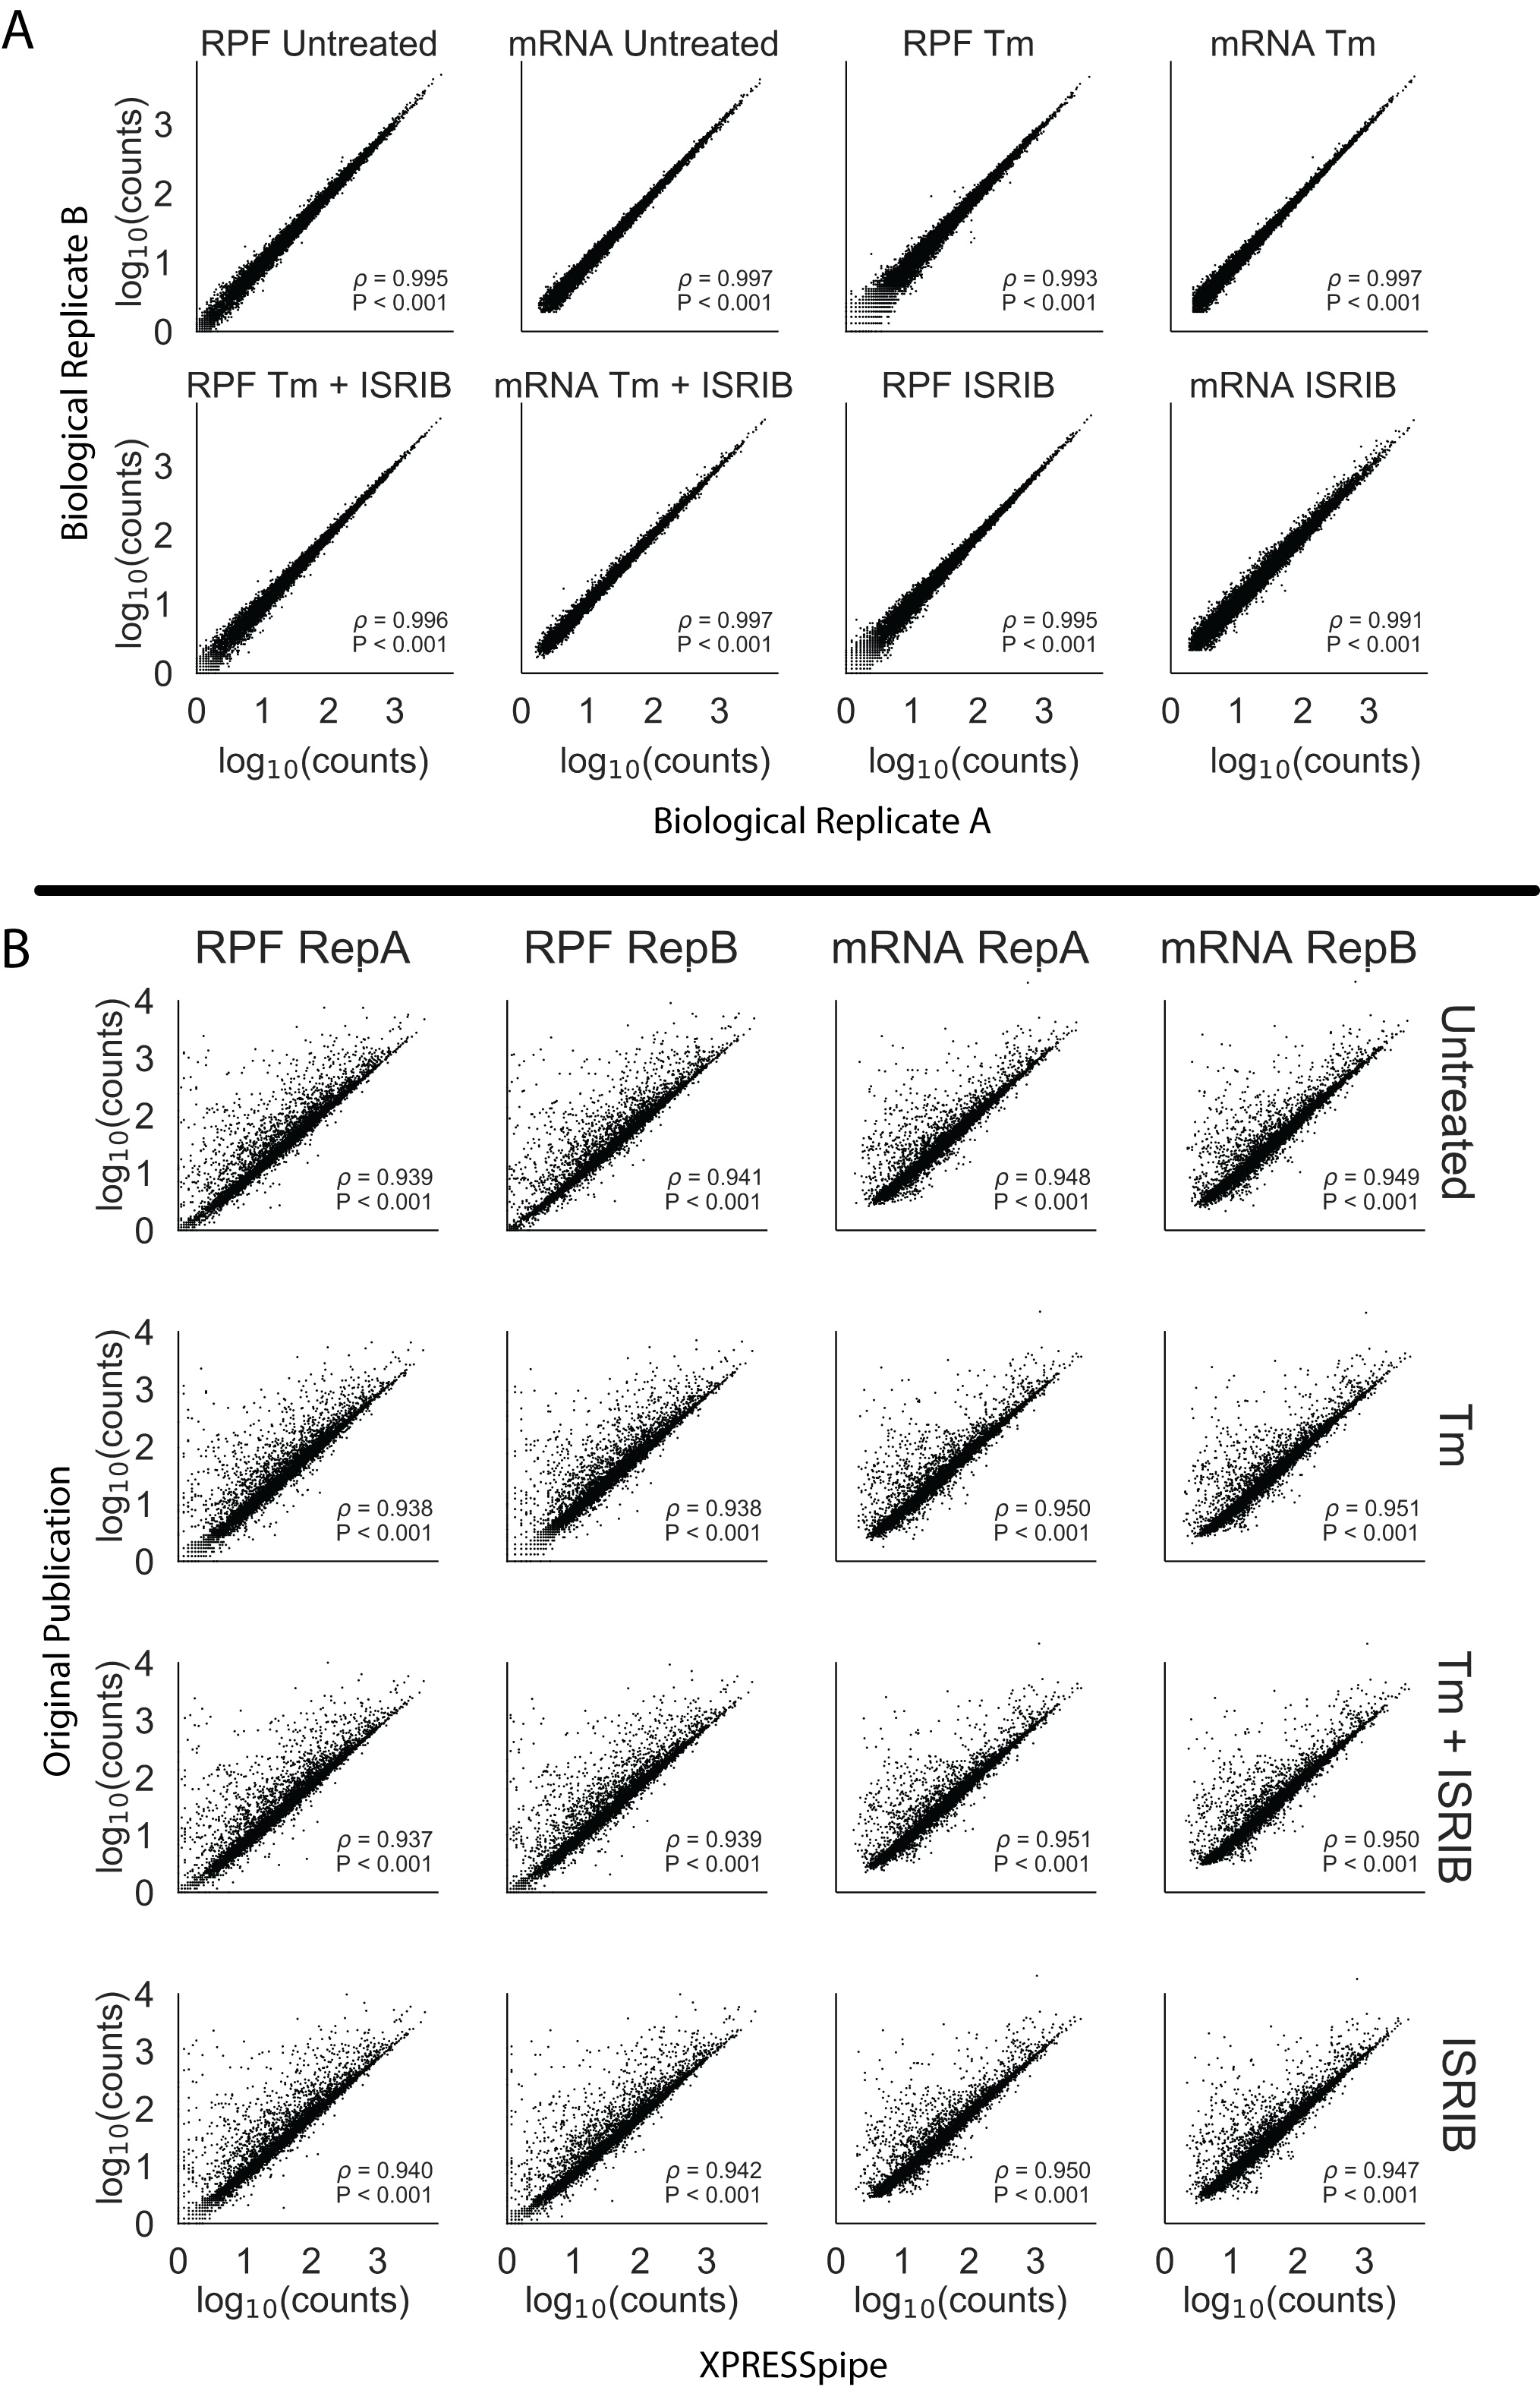
\includegraphics[width=180mm]{figures/xpresspipe_supplement3.png}
  \caption{A) Fold change for each drug condition compared to untreated for the de-duplicated ribosome profiling and RNA-seq data. ISR canonical targets passing fold change and significance threshold during Tm conditions are highlighted in magenta. All translationally down-regulated genes passing fold change and significance threshold during Tm conditions are highlighted in green. B) Changes in log\textsubscript{2} Translation Efficiency compared to Untreated for each drug condition for each of the canonical ISR genes passing previous discussed thresholds. C) IGV plot for ENPP5 for all ribosome profiling samples show read coverage across the transcript. D) IGV plot for ATF4 for all ribosome profiling samples show read coverage across the transcript.}
  \label{fig:supplement3}
\end{figure}

\end{document}
